
\documentclass[12pt]{article}
\usepackage{enumitem}
%\usepackage{paralist}
\usepackage{amssymb}
\usepackage{url}
\usepackage{tabulary}
\usepackage[ruled,boxed]{algorithm2e}
\usepackage{graphicx,epsfig,fancybox,amsthm}
\usepackage{verbatim}
\usepackage{caption}
\usepackage{subcaption}
\newtheorem{theorem}{Theorem}[section]
\newtheorem{lemma}[theorem]{Lemma}
\newtheorem{proposition}[theorem]{Proposition}
\newtheorem{corollary}[theorem]{Corollary}
\newtheorem*{defi}{Definition}
\newtheorem{exmp}{Example}[section]
\setcounter{AlgoLine}{0}
\setlength{\textwidth}{6.5 in}
\setlength{\textheight}{9 in}
\setlength{\topmargin}{-1.0 in}
\setlength{\oddsidemargin}{0.0 in}
\setlength{\evensidemargin}{0.0 in}
\begin{document}
%------------------------------------------------------------
\newcommand {\nwline}   {\hfill\break}
\newcommand {\closeup}  {\vspace*{-0.2in}}
\newcommand {\hLine}[1] {\begin{center}\rule{#1}{0.25mm}\end{center}}

\newcommand {\ol}[1]    {\overline{#1}}
\newcommand{\Prob}[1]   { {\bf \mathrm{Prob}} \left[ #1 \right] }
\newcommand{\Var}[1]    { {\bf \mathrm{Var}} \left[ #1 \right] }
%------------------------------------------------------------


\fbox{
    \begin{minipage}[t]{6.0in}
    \begin{description}
    \item[Title:]	Thesis Report

    \item[Project Title:] k-Tree Bound on Probabilistic Connectivity of Underwater Sensor Network.
    \item[Name:]	Md Asadul Islam

    \item[Date:]	\today

    \end{description}
    \end{minipage}
}
%------------------------------------------------------------

\begin{abstract}

\begin{comment}
Note that a paper's abstract is intended to be a concise highlevel
description of the contents of the paper. It implicitly defines a road
map of the important aspects of the paper (without referring to exact
section numbers) and it should do a good job in mentioning all such
important aspects in a coherent way.


\end{comment}
\end{abstract}

% ------------------------------% Here is the main document


\section{Introduction}


Underwater Sensor Networks (UWSNs) is a promising tool  because of its remote monitoring and control technology. Application domain of such UWSNs can be military surveillance, disaster prevention, assisted navigation, offshore exploration, tsunami monitoring, oceanographic data collection, to mention a few. Most of the above mentioned applications requires UWSNs nodes move
freely with water currents. Thus, node locations at any instant need to be specified probabilistically. When connectivity among some of the sensor nodes is required to perform a given function, the problem of estimating
the likelihood that the network achieves such connectivity arises. In this thesis, we formulates some parameterized probabilistic connectivity problem that serves this purpose when the network contains both sensor nodes and relay nodes.

 In this chapter, we introduce some of such research problems. We also
give an overview of UWSNs, and discuss how such
problems can be tackle.
\subsection{Introduction}
Underwater Sensor Networks (UWSNs) is a prominent network paradigm which consist of variable number of sensor nodes. Primary objective of UWSNs is collaborative monitoring and resource exploration. Underwater communication is using since the World War II, when hydro-phone developed in United States to communicate with submarine \cite{quazi1982underwater} but still there are many unexplored area in UWSNs which need to be addressed.  Recently UWSNs research is intensified because there are many important applications of underwater sensing networks \cite{akyildiz2005underwater}  \cite{heidemann2012underwater} \cite{climent2014underwater}. According to \cite{heidemann2012underwater} the application domain of UWSNs can be classified as

\begin{itemize}[noitemsep]
\item Scientific applications such as observe geological processes on the ocean floor, determine water characteristics e.g. temperature, salinity, oxygen levels, bacterial and other pollutant content, dissolved matter, counting or imaging animal life e.g micro-organisms, fish or mammals,coral reef \cite{bromage2007sea}.

\item Industrial applications monitor and control commercial activities, such as determine route for underwater cable,
underwater equipment related to oil or mineral extraction, underwater pipelines or commercial fisheries. Industrial applications often involve control and actuation
components as well.

\item Military and homeland security applications involve securing or monitoring port facilities or ships in foreign harbours, de-mining and communication with submarines and divers.

\item Humanitarian applications involves search and survey missions e.g. sunken ships,  digester prevention e.g. tsunami warning to coastal areas \cite{cruz2008ocean}, identify hazards on the seabed, locate dangerous rocks or shoals in shallow waters, mooring positions, submerged wrecks etc.
\end{itemize} 
 
Different types of UWSNs deployment is used in-order to serve above diverse types of applications. According to \cite{heidemann2012underwater}, UWSNs deployment can be classified as static, semi-mobile and mobile.
\begin{itemize}
\item Static deployment can be considered as two-dimensional architecture of UWSNs where nodes are attached to docks,  buoys, or underwater ground. In this type of network all nodes can communicate with each other, so the network is always connected until battery depleted of some nodes. Typical application of this type of UWSNs can be underwater plates in tectonics monitoring\cite{freitag2002acoustic}, identify hazards on seabed.
\item In semi-mobile deployment, nodes are suspended from buoy or they can be anchored to the seabed by strings.  So nodes in the semi-mobile UWSNs can move but their movement are limited. The network topology of semi-mobile deployment is static for long duration which promotes connectivity. However the connectivity changes with water currents, subsurface waves, whirls etc. Semi-mobile UWSNs can be considered as static three dimensional architecture of UWSNs. Semi-mobile UWSNs may be used for surveillance applications or monitoring of ocean phenomena e.g. ocean bio–geochemical processes, water streams, pollution.

\item Mobile UWSN consists of low powered gliders or unpowered drifters. Nodes are subject to large scale movement. Mobility are useful to cover large area of ocean with limited hardware component but it raises many challenges in node localization and network connectivity.
\end{itemize}
 
 As there are vast diversity of applications of UWSNs and challenges encountered in UWSN design, extensive research work spanning all five layers of the internet protocol stack appears in the literature. Now, we talk about the design of a protocol stack for underwater acoustic
communication. For more information you can read research works \cite{cui2006challenges}, \cite{heidemann2012underwater}, \cite{akyildiz2005underwater} and \cite{benson2006design}.
\begin{itemize}
\item  \textbf{Physical layer: }
Electromagnetic communication such as radio and optical signal quickly absorbs by  water make acoustic communication preferable for UWSNs communication. Path loss due to  high attenuation of acoustic wave causes by the distance between transmitter and receiver, surface-bottom reflection and refraction etc. and geometric spreading, man maid noise and ambient noise, multi-path propagation, high delay due to low data rate and Doppler effect are the challenges for physical layer design.

Frequency shift keying(FSK) and non-coherent detection which are very effective for robust communication with low bit rates were using early systems such as for commercial modems (e.g. Telesnor series\cite{green2010acoustic}) and in research prototype (e.g. micro modem development at WHOI\cite{singh2009acoustic})

Non-coherent technique need phase tracking,
which is a very difficult task in underwater environment.
On the contrary coherent modulation techniques does not need such tracking and have been developed for long-range, high-throughput systems \cite{stojanovic1993adaptive} (such as phase shift keying (PSK) and quadrature amplitude (QAM)) and are using today's ‘high-speed’ communications.
\item \textbf{Data Link Layer: }
Multiple access techniques are developed to allow devices to access a common
medium, sharing the scarce available bandwidth in an efficient and fair way.
Channel Access Control in an underwater sensor network poses additional
challenges such as long delays, frequency-dependent attenuation and the relatively
long reach of acoustic signals due to the peculiarities of the underwater channel, in particular.

Time division multiple access (TDMA) and frequency division multiple access (FDMA) were using at the early stage of development of UWSNs. Channel separation in FDMA leads some inefficiency and all user in TDMA need to be synchronised make them unsuitable for UWASs.


In code division multiple access CDMA signals that coexist in both time and frequency
can be separated using specifically designed codes in combination with signal
processing techniques, allows multiple devices to transmit
simultaneously over the entire frequency band. effectiveness on multi-path fading and not require slot synchronization makes CDMA and attractive choice for UWSNs link layer protocol.

ALOHA is a class of MAC protocols that do not try to prevent packet
collision, but detect collision and retransmit lost packets. In the
underwater acoustic environment, ALOHA protocols are affected by low
efficiency, mainly due to the slow propagation of the acoustic channel.
Additionally, the need for retransmissions increases the power
consumption of sensors, and ultimately reduces the network lifetime.

Carrier sense multiple access (CSMA) protocols are aimed at reducing
the packet retransmissions, by monitoring the channel state: if the
channel is sensed busy, packet transmission is inhibited so as to prevent
collisions with the ongoing transmission. If the channel is sensed free,
transmission is enabled. However this approach, although it prevents
collisions at the sender, does not avoid collisions at the receiver due to
the hidden and exposed terminal problems.

\item \textbf{Network Layer: }
Network layer is responsible for delivering data from source to destination, possibly over multi-hop basis. Recent years tremendous amount of research is going on physical layer and link layer but there are many unexplored area in network layer.

Early work on routing is vector Based Forwarding \cite{xie2006vbf} where data packets are forwarded along redundant and interleaved paths from the source to sink. This helps in tacking the problems of packet losses and node failures. Forwarding path is nominated by the routing vector from source to destination. All the nodes receiving the packet computes their positions by measuring its distance to the forwarder. The forwarding path is virtually a routing pipe and the nodes inside this pipe are eligible for packet forwarding. A distributed protocol is proposed by Pompili et al. [31], which is applicable for both delay sensitive and delay-insensitive applications and allow nodes to select the next hop with the objective of minimizing the energy consumption while taking into account the specific characteristics of acoustic propagation as well as the application requirements. A depth based routing is proposed in \cite{yan2008dbr}. When a node wants to send a data packet, it senses own relative current position from the surface and place its value in the header and then broadcasts. The receiving node calculates its own depth position and compares this value with the value embedded. If the value is smaller then forward the packet otherwise discard it. The performance of this protocol worse if the area is sparse and affected by packet loss.

\item \textbf{Transport layer: }
A transport layer protocol is needed in underwater acoustic sensor networks not
only to achieve reliable collective transport of event features, but also to perform
flow control and congestion control. The primary objective is to save scarce
sensor resources and in-crease network efficiency. A reliable transport protocol
should guarantee that the applications are able to correctly identify event
features estimated by the sensor network. Congestion control is needed to
prevent the network from being congested by excessive data with respect to the
network capacity, while flow control is needed to avoid that network devices
with limited memory are overwhelmed with data transmissions.


Several solutions have been proposed to address the transport layer problems
in UWSNs. For example, Event-to-Sink Reliable Transport (ESRT) protocol is proposed to achieve reliable event detection with minimum energy expenditure. However, the ESRT mechanism relies on spatial
correlation among event flows which may not be easily leveraged in underwater
acoustic sensor networks. Hence, further investigation is needed to develop
efficient transport layer solutions
\end{itemize}
 
\begin{comment}  See e.g. survey article of \cite{partan2007survey} and \cite{climent2014underwater} and  chapters in \cite{xiao2010underwater} and \cite{otnes2012underwater}. Also there are some real-world research include \cite{jaffe2006sensor}, \cite{evolo} \cite{rice2000evolution} \cite{roy2006wide} \cite{pu2013comparing}
 \end{comment}

 Connectivity is an important issue for UWSN in-order to perform localization \cite{zhou2010efficient}, \cite{zhou2011scalable},\cite{erol2011performance}, routing \cite{noh2013vapr},\cite{ying2011combining},\cite{lee2010pressure}. In this thesis, we are interested to measure the connectivity of UWSN. We are considering a  semi-mobile and mobile UWSNs. Our interest is to develop methodologies that allows a designer to analyze the likelihood  that a network is connected and the connectivity we are interested, can be All node connectivity: every node is connected with sink and connectivity with $N_{req}$: compute the probability that at least $N_{req}-1$ nodes is connected with sink node.
 
 
 The rest of chapter is organized as follows. In section 1.2 we introduce different class of connectivity  problems. In section 1.3 we give an overview of some
important literature in this area. In section 1.4 we outline thesis
contributions and organizations.
\subsection{Literature Review}
 A review of some published research work in this field indicates the following categories of research directions.
 \begin{itemize}
 \item[a.] Connectivity and coverage issue for underwater sensor network.
 \item[b.] $k$-tree and partial $k$-tree.
 \item[c.] Mobility models for underwater sensor network.
 \end{itemize}
 \subsubsection{Connectivity and coverage }
 In this section, we are going to describe some literature discuss the connectivity and coverage issue of underwater wireless sensor network.
 \begin{itemize}
 \item[1.] Authors in \cite{senel2013autonomous} proposes a UWSN distributed node deployment strategy where they drop the nodes on the water surface. Maximize coverage and guaranteed connectivity from initial deployment was their primary goal. They finds the connected dominating set of initial deployment by using using a distributed leader election algorithm at 2-$D$ plane. After that they adjust the depth of all dominatee which maintain the connectivity with dominant node by stretched along $z$ axis as much as possible until their sensing ranges do not overlap to maximize coverage. They claim  that connectivity is guaranteed regardless of the transmission and sensing range
ratio with a coverage very close to a coverage-aware deployment
approach.

 \item[2.] In \cite{akkaya2009self} authors propose a distributed node deployment scheme which can increase the initial network coverage in an iterative basis. They assuming that the nodes are initially deployed at the bottom of the water and can only move vertically in 3-D space. The idea is to relocate the nodes at different depths based on a local agreement in order to reduce the sensing overlaps among the neighbouring nodes. Redundancy is observe by one  of the node called Leader. It utilizes vertex colouring problem formulation in-order to determine coverage overlap. The nodes continue to adjust their depths until there is no room for improving their coverage. This work improves the coverage significantly but
does not guarantee any connectivity. It is only claimed that
with a certain transmission range and sensing range ratio, the
connectivity can also be ensured. While this has been shown
to be the case with a certain number of nodes and ratio, the
approach certainly cannot guarantee the connectivity for all
cases.
 
 \item[3.] Authors in \cite{ammari2010study} analyse  the connectivity and k-coverage issues in 3D WSNs, where each point is covered by at least k sensors. They proposes  the Reuleaux tetrahedron model to characterize $k$-coverage of a $3D$ field and investigate the corresponding minimum sensor spatial density. They compute the connectivity of 3D k-covered WSNs. They prove that $3D$ $k$-covered WSNs can sustain a large number of sensor failures based on conditional connectivity and forbidden faulty sensor set. Finally they provide a measure of connectivity and
fault tolerance of $3D$ WSNs based on an accurate characterization of $k$-coverage of $3D$ fields.

\item[4.] In \cite{Nazrul2008} authors tackling the problem of determining how to deploy minimum number of sensor nodes so that all points inside the network is within the sensing range of at least one sensor and all sensor nodes can communicate with each other, possibly over a multi-hop path. They used sphere-based communication
and sensing model. They place a node at the center of each virtual cell created by truncated octahedron-based tessellation.  The paper concludes that truncated octahedrons yield the best results for coverage. Using the same polyhedron, connectivity is guaranteed if the transmission range of the nodes is at least 1.7889 times the sensing range.
 \end{itemize}
 \subsubsection{$k$-tree and partial $k$-tree}
\begin{itemize}

 \item[1.] In \cite{Beineke1971}, authors introduce the class of $k$-tree, $k\geq1$, as generalization of trees as follows. The complete graph on $k$ vertices, denoted $k_ k$ , is a $k$-tree. Furthermore, if $G$ is a $k$-tree then so is the graph obtained from $G$ by adjoining a new vertex, and making it adjacent to every vertex in a complete subgraph on $k$ vertices of $G$. Partial $k$-trees are subgraph of $k$-trees. 
 \item[2.] Recently in \cite{shangin2014heuristics} authors introduce a problem to find a minimum weight spanning $k$-tree in a complete weight graph. The above problem is known to be NP-hard problem. They proposes four heuristics to solve above problem. Finally they compare their proposed algorithms with known heuristics and exact algorithms.
\end{itemize}
\subsubsection{Mobility Models}
\begin{comment}
Several experimental and analytical results in oceanography literature have
shaped our current understanding of mobility for underwater sensor networks. Of the vast literature existing in the field, we recall the following early landmark
results. 

\begin{itemize}
\item[1.]In \cite{bower1989evidence}, the authors report on several observations collected in the Gulf Stream using thirty-seven RAFOS drifters launched off Cape Hatteras. Mobility of the free floating drifters are tracked for 30 or 45 days. In \cite{bower1991simple}, the author describes a 2-dimensional kinematic model of a meandering jet. The model captures the striking patterns of cross-stream and vertical motion associated with meanders observed in \cite{bower1989evidence}.

\item[2.] Investigations and results obtained in the above directions
have been valuable for networking researchers approaching the challenge of modelling the mobility of underwater sensor networks. In \cite{caruso2008meandering}, the authors adopt a kinematic model for capturing the effect of meandering sub-surface currents and vortices of free floating sensor nodes. The model, called the meandering
current mobility model, is useful for large coastal environments that span several kilometers. It captures the strong correlations in mobility of nearby sensor nodes.
Using simulation, the authors investigate several network connectivity, coverage, and localization aspects.
\item[3.] In \cite{luo2009double}, \cite{luo2012double}, the authors consider sensor nodes with movement capability. Each node incurs both uncontrollable and controllable mobility (abbreviated as U-mobility and C-mobility). Using a grid layout that divides a geographic area into cells, the authors adopt a probabilistic U-mobility model. The model takes into consideration two types of effects: local variety effects (caused by
reefs, turbulence), and main circulation effects (caused by wind, salinity). Using such model, the authors present an energy efficient approach for satisfying network coverage requirements.
\end{itemize}
In this paper, we adopt a simple probabilistic locality
model where the geographic area under consideration is
partitioned into disjoint regions (rectangles) using a grid
layout. In our model, the use of a high grid resolution
(i.e., a layout with small regions) can potentially give
accurate results at the expense of decreased solution
efficiency. We assume that one can utilize a physical
model of underwater currents to compute the probability
that a sensor node is located at a given region during
some time interval of interest. Using such probability
distribution, one obtains a probabilistic graph model of
the network.

Our work here formalizes two problems, denoted
A-CONN and S-CONN, that call for determining the
likelihood that a probabilistic graph is entirely or partially
connected. Our main contribution is an efficient
dynamic programming algorithm to solve both problems
on tree-like networks. The algorithm can be used to
derive lower bounds on the solution of any arbitrary
probabilistic network. Our devised algorithm extends a
result in \cite{ProfEhab} to compute the probability that a given
sequence of nodes in a probabilistic network forms a
simple connected path. To the best of our knowledge,
both the problems formulation and devised algorithm are
\end{comment}
\subsection{Network Model and Problem Formulation}
In this section, we present a network model that deals with arbitrary topologies where each node is located into a set of regions with probability. We also present four fundamental connectivity problems, denoted by $A-CONN$, $A-CONN$ with $Relays$, $S-CONN$ and $S-CONN$ with $Relays$ . In two of our problem formulation we used relay nodes in addition to sensor nodes which do not have the sensing capability but helps to improve overall network performance.\\ 

The first problem is all sensor nodes connectivity problem:
\begin{defi}[\textbf{the $A-CONN$ Problem}]
\normalfont
Given
\begin{itemize}[noitemsep]
\item a UWSN $G$.
\item a set of sensor nodes $V_{sense}$.
\item a sink node $s$. So the set of all node $V=\{V_{sense}\cup s\}$
\item  a set of regions  $R_v=\{r_{(v,1)},r_{(v,2)},....\}$  with probability $p(r_{(v,i})$ where $i=1,2,...$ for each node $v\in V$
\item transmission radius $R_{tr}(v)$  for node $v\in V$.
\end{itemize} compute the probability $Conn(G)$ that the network in a state where sink node $s$ can reach all sensor nodes. $\blacksquare$

\end{defi}
The second problem is all sensor nodes connectivity problem with the present of relay nodes:
\begin{defi}[\textbf{the $A-CONN$ with $Relays$ Problem}]
\normalfont
Given
\begin{itemize}[noitemsep]
\item a UWSN $G$.
\item a set of sensor nodes $V_{sense}$.
\item a sink node $s$.
\item a set of relay nodes $V_{relay}$. So the set of all nodes $V=\{V_{sense}\cup s \cup V_{relay}\}$.
\item  a set of regions  $R_v=\{r_{(v,1)},r_{(v,2)},....\}$  with probability $p(r_{(v,i})$ where $i=1,2,...$ for each node $v\in V$.
\item transmission radius $R_{tr}(v)$  for node $v\in V$.
\end{itemize} compute the probability $Conn(G,V_{relay})$ that the network in a state where sink node $s$ can reach all sensor nodes. $\blacksquare$
\end{defi}
The third problem is the subset sensor nodes connectivity problem:
\begin{defi}[\textbf{the $S-CONN$ Problem}]
\normalfont
Given
\begin{itemize}[noitemsep]
\item a UWSN $G$.
\item a set of sensor nodes $V_{sense}$.
\item a sink node $s$. So the total number of nodes in the network $V={\{V_{sense}\cup s\}}$
\item an integer $n_{req},n_{req}\leq |V_{sense}|$
\item  a set of regions  $R_v=\{r_{(v,1)},r_{(v,2)},....\}$  with probability $p(r_{(v,i})$ where $i=1,2,...$ for each node $v\in V$.
\item transmission radius $R_{tr}(v)$  for node $v\in V$.
\end{itemize} compute the probability $Conn(G,n_{req})$ that the network in a state where sink node $s$ can reach a subset of sensor nodes having atleast $n_{req}$ sensor nodes. $\blacksquare$
\end{defi}
Finally the fourth problem is the subset of sensor nodes connectivity problem with the present of relays nodes in the network:
\begin{defi}[\textbf{the $S-CONN$ with $Relays$ Problem}]
\normalfont
Given
\begin{itemize}[noitemsep]
\item a UWSN $G$.
\item a set of sensor nodes $V_{sense}$.
\item a set of relay nodes $V_{relay}$.
\item a sink node $s$. So the total number of nodes in the network $V={\{V_{sense}\cup s\cup V_{relay}\}}$
\item an integer $n_{req},n_{req}\leq |V_{sense}|$
\item  a set of regions  $R_v=\{r_{(v,1)},r_{(v,2)},....\}$  with probability $p(r_{(v,i})$ where $i=1,2,...$ for each node $v\in V$.
\item transmission radius $R_{tr}(v)$  for node $v\in V$.
\end{itemize} compute the probability $Conn(G,n_{req})$ that the network in a state where sink node $s$ can reach a subset of sensor nodes having atleast $n_{req}$ sensor nodes. $\blacksquare$
\end{defi}
We now draw following remarks about the above problems
\begin{itemize}
\item[1.] The $A-CONN$ is the core problem which is the modified to formulate $A-CONN$ with $Relays$, $S-CONN$ and  $S-CONN$ with $relays$ problems.
\item[2.] The $A-CONN$ problem is a special case of $A-CONN$ with $Relays$ problem. If the input UWSN $G$ consists of only sensor nodes then the connectivity provided by $A-CONN$ will be same as the connectivity provided by $A-CONN$ with $Relays$. But after adding relay nodes the connectivity provided by $A-CONN$ with $Relays$ for graph $G$ will be higher than the connectivity provided by $A-CONN$ for graph $G$.
\item[3.] The $A-CONN$ is a important special case of the $S-CONN$ problem where $n_{req} \leq |V_{sense}|$. In the $A-CONN$ problem, the network is operating if the sensor node $s$ can reach all sensor nodes. On the other hand The $S-CONN$ problem, the network is operating if sink $s$ can reach a subset having at least $n_{req}$ sensor nodes.
\item[4.] Similarly the $S-CONN$ problem is a special case of $S-CONN$  with $Relays$ problems.
\end{itemize}


\subsection{Thesis Contribution and Organization}
\subsection{Summary}
\section{Background on k-tree}
\subsection{Introduction}
In this chapter we started by providing some background on $k$-tree and partial $k$-tree. We define perfect elimination sequence which is important to construct $k$-trees from a given set of nodes with their probabilistic locality set. We provide two algorithm in-order to construct $1$-tree and $2$-tree. Finally, we present some idea on how to construct $3$-tree and draw some conclusions.
\label{sec:ktree}
\subsection{Definition of k-tree}
In this section, we define clique, $k$-tree and we present  partial $k$-tree and their classes.\\
\begin{defi}
A clique is a set of vertices that induce a complete subgraph of a graph \(G\). A clique with \(k\) vertices is considered to be a \(k\)-tree. 
\end{defi}
 \begin{defi}Treewidth is a parameter which is use to measure how a graph is ``tree like'' or ``close to being a tree''. Treewidth of \(k\) tree is \(k\).
\end{defi}
\begin{defi}
\normalfont
The class of  \(k\)-tree can be  defined recursively as follows: 
\begin{itemize}[noitemsep,nolistsep]
 \item The complete graph on $k$ vertices is a $k$-tree.
 \item Lets \(G_n\) is a \(k\)-tree  with $n$ vertices where $n\geq k$. Then we can construct a $k$-tree $G_{n+1}$ of $n+1$ vertices by adding a vertex adjacent to exactly $k$ vertices, namely all vertices of a $k$ clique of $G_n$. $\blacksquare$
\end{itemize}

\end{defi}
  A partial \(k\)-tree is a graph which contains all the vertices and subset of edges of a $k$-tree.  Partial \(k\)-trees are rich class of graph. Forest is an example of partial 1-tree. Series-parallel graphs and chordal graphs are subfamily of partial \(2\)-trees. Also Halin graphs, Nested SAT and IO-graphs are subclasses of partial \(3\)-trees. 
  
   Several graph problem that are NP-complete on general graphs have polynomial time algorithms for graphs with treewidth bounded by a constant. Any polynomial time algorithm for graphs of bounded treewidth is a polynomial time algorithm for partial \(k\)-tees. So partial \(k\)-trees are useful as they might be seen as a tool to gain more insight in graphs of bounded treewidth.

  \begin{exmp}
  \normalfont
  Fig. 1 depict a partial $2$-tree. The complete graph of $2$ vertices namely $v_1$ and $v_2$ is a $2$-tree. Then we added vertex $V_3$ which is adjacent to both $v_1$ and $v_2$ is a $2$-tree of $3$ vertices. Finally a vertices $s$ is added to the clique $v_1v_2$ to form the $2$-tree with $4$ vertices.$\blacksquare$
  \end{exmp}
\subsection{Perfect Elimination Sequence}
A perfect elimination sequence (PES) in a graph is an ordering of the vertices of the graph such that, for each vertex $v$, $v$ and the neighbors of $v$ that occur after $v$ in the order form a clique. In-order to find PES we need simplicial vertex.
\begin{defi}[Simplicial Vertex]
\normalfont
A simplicial vertex of a graph $G$ is a vertex $v$ such that the neighbours of $v$ form a clique in $G$. Clearly, if $G$ has a PES, then the last vertex in it is simplicial in G.$\blacksquare$
\end{defi}
\begin{comment}
\begin{defi}[Chordal Graph] 

A graph is chordal if its cycles of four or more vertices has a chord, which is an edge thet is not part of the cycle but connect two vertices of the cycle. $\blacksquare$
\end{defi}

\begin{lemma}
A chordal graph is either complete or has at least two non adjacant simplical vertex\cite{heggernes2006treewidth}.
\end{lemma}
A graph is chordal if and only if it has a PES. There is a corollary that every $k$-tree is a chordal graph \cite{heggernes2006treewidth}. So there is a perfect elimination ordering for every $k$-tree. 
Now in-order to find PES we need to repeat the following step until no simplicial vertices are left: Find a simplicial vertex and remove it from the graph.
If the graph is chordal, there will be a simplicial vertex at each step, by the
above lemma. Therefore, if the remaining graph is not empty at the end of
this process, then we can conclude that the input graph is not chordal. If no
vertices remain at the end of the process, then the order in which the vertices
are removed is called a perfect elimination order.
\end{comment}
\begin{exmp}
\normalfont
In fig. 1 we show that there are two simplicial vertices, $v_1$ and $s$. But $s$ is our sink node so we are not eliminating $s$. So After elimination of $v_1$, we will be able to eliminate either $v_2$ or $v_3$. So the PES will be either $v_1,v_2$ or $v_1,v_3$.$\blacksquare$
\end{exmp}
\section{Extracting a k-tree}
In this section, we are going to describe how we construct a $k$-tree from a set of given UWSN node where each node can be located into a set of regions.
\subsection{Extracting 1-tree}
We describe how we construct $1$-tree for given a set of nodes.

We are given a set of nodes $V$ where each nodes is located into a set of regions. The function OneTree() construct a greedy 1-tree, $Tree(V,E)$ which has the heighest connectivity.
\begin{itemize}[noitemsep]
\item Step 1: $N$ is a set which is initialize by $\{V\setminus sink\}$ and $T$ is another set which is initialized by $sink$ node. $E$ is a empty edge set.
\item Step 2: repeat the following steps until $N$ is empty.
\item Step 3: if $p\in N$ and $q\in T$ are two nodes which has a connectivity probability greater than or equal to any other remaining pair. For pairs we indicate one node from set $N$ and another node from set $T$
\item Step 4: add the edge $e(p,q)$ to $E$.
\item  Step 5: delete node $p$ from set $N$ and add $p$ to $T$. 
\item  Step 6: Finally the algorithms return the tree $Tree(V,E)$
\end{itemize}
 
\begin{algorithm}
\KwIn{ $V$ is a set of nodes where each node is located into a set of probable regions}
\KwOut{A $1$-tree $Tree(V,E)$}

\nl \textbf{Initialization: } $N$ and $T$ are two sets of nodes where $N$ is initialized by all given nodes in $V$ except the sink node and $T$ is initialized by the sink node and $E$ is an empty edge set.\\
\nl \While{$N!=\emptyset$}
{
\nl $p\in N$ is a node and $q\in T$ is another node where  the connectivity probability between node $p$ and $q$ is higher or equal to another pair.\\
\nl add $(p,q)$ to $E$.\\
\nl delete node $p$ from $N$ and add $p$ to $T$\\
}
\nl Return{$Tree(V,E)$}
\caption{Function OneTree($V$)}
\end{algorithm}
\subsection{Extracting 2-tree}
In-order to extract $2$-tree, we use the $1$-tree skeleton.
We use two functions check($Tree$) and TwoTree($Tree$,$Tree_1$) to convert  1-tree to 2-tree.
\begin{algorithm} 
\Indm
\KwIn{ a UWSN $T(V,E)$ is a partial $2$-tree where each node, $v\in V$  can be located into a set of regions $R_v=\{r_{(v,1)},r_{(v,2)}...\}$ with probability,  $\{p(r_{(v,1)}),p(r_{(v,2)})...\}$ and $(x,y)\in E$ if $x\in V$ can be located one of it's locality set and $y\in V$ can be located one of it's locality set, so that they reach each other.}
\KwOut{ $flag$ }

%\noline
\Indp
\nl \textbf{Initialization:} set $counter =0$ and $flag=false$ \\

\nl\ForEach{node $v\in V$ and $counter<|V|$}
{
\nl \If{$deg(v)==1$}{
\nl  \If{$e(v,v_{t})\in E$}{
  $E=E\setminus e(v,v_{t})$; $V=V\setminus v$; $counter=0$
}
}
\nl \ElseIf{$deg(v)==2$}{
\nl \If {$e_1(v,v_1)\in E$ and $e_1(v,v_2)\in E$}{
 $E=E\setminus \{e_1(v,v_1)\cup e_2(v,v_2)\}$ ;$V=V\setminus v$; $counter=0$}
\nl \If{ $e(v_1,v_2)\not \in E$ }{  $E=E\cup e(v_1,v_2)$ }
}
 \Else {
\nl $counter=counter+1$}
}
 \If{$|V|=0$}{
\nl set $flag$=$true$
}
 \nl \Return $flag$
\caption{Function Check$(T(V,E)$}
\end{algorithm}
\subsubsection{Function Check}
The check function take a tree as a input and check that whether it's a partial 2-tree or not. If the input tree is a partial 2-tree then it returns $true$ otherwise it returns $false$.
\begin{itemize}[noitemsep]
\item Step 1: it initializes a $counter$ by 0 which help to terminate infinite looping and $flag$ by $false$.
\item Step 2: it's iterates from step 3 to step 10 for each node $v\in V$ and $counter$ less than equal to the size of $V$. The $counter$ is going to be always less than the size of $V$ if $T(V,E)$ a partial 2-tree. 
\item Step 3: it finds the number of edges associated with node $n$ in $T(V,E)$ by simply searching through the edge set of $T(V,E)$. This value indicates the degree $deg$ of $v$. If $deg(v)$ is equal to one then it is safe to remove the node $v$ and associated edges from $T(V,E)$.
\item Step 4: it find the edge $e(v,v_t)$ associated with node $v$ where $v_t$ is the neighbour of $v$. It removes  $e(v,v_t)$ from the edge set $E$ and $v$ from vertices set $V$. Finally it reset the $counter$ to make sure that upto this point it's a partial $2$-tree.
\item Step 5: if the degree $deg$ of $v$ is two then it is also safe to remove the vertices and associated edges.
\item Step 6: so in-order to remove the node $v$, it's finds the edges $e_1(v,v_1)$ and $e_2(v,v_2$ associated with $v$ by searching the edge set $E$ of $T(V,E)$. Also it finds the neighbours $v_1$ and $v_2$ of $v$. Lastly, it removes $e_1(v,v_1)$ and $e_2(v,v_2)$ from the edge set $E$ and $v$ from the vertices set $V$. It reset the $counter$ to make sure that after upto deleting this node, the tree maintains the property of 2-tree.
\item Step 7: it search the edge set $E$ of $T(V,E)$ for an edge between the neighbour's of $v$ i.e. an edge between $v_1$ and $v_2$. If there is no edge then it add an edge$e(v_1,v_2)$ to $E$.
 
\item Step 8: if step 3 and step 5 are false then it increment the value of $counter$ by one. If each node has a degree more than 2 then the tree is not going to be a partial 2-tree. We are incrementing the $counter$ so that in above situation it will terminate from infinite looping.
\item Step 9: after exiting from the loop it check $|V|$ is empty or not. $|V|$ empty means we are able to delete all nodes so $T(V,E)$ is a partial 2-tree and it assign $true$ to the $flag$.
\item Step 10: Finally it returns the $flag$.
\end{itemize}
\subsubsection{Function TwoTree}
We are given $T(V,E)$, a one tree generated by function OneTree() and a edge set $E_1$ which contains all possible edges between vertices set $V$ excluding $E$. That is $E\cap E_1=\emptyset$. The function TwoTree() select high probable edges and from $E_1$ and check whether or not after adding that edge to $T(V,E)$, it hold the property of 2-tree. If so then it add that edge to $E$ and delete it from $E_1$.


\begin{itemize}[noitemsep]
\item Step 1: in \cite{Elmallah88partitioningthe} authors shows that if $G$ is a $k$-tree on $n$ vertices and $m$ edges then $m = kn - k(k +1)/2$ and for $2$-tree $m=2n-3$. We iterates until the size of $E$ less than $2*|V|-3$.
\item Step 2: select an edge $e$ from $E_1$ which has the connectivity value greater than or equal to any other edge in $E_1$.
\item Step 3: use the check function to check after adding this edge to $T(V,E)$, it's still going to be a partial 2-tree. 
\item Step 4: if the above condition hold then it will add the edge to the edge-set $E$ of $T(V,E)$.
\item Step 5: it remove the edge from the edge-set $E_1$
\item Step 6: it returns the partial 2-tree constructed by this greedy technique.
\end{itemize}

\begin{algorithm}
\KwIn { $T(V,E)$ is a $1$-tree and $E_1$ is a edge set where $E\cup E_1$ is the set of all possible edges between vertices $V=\{v_1,v_2,.....,v_n\}$ and $E\cap E_1=\emptyset$  }
\KwOut{A partial $2$-tree.}
\nl \While{$(|E|<2*|V|-3)$}
{
\nl select a edge $e(v_1,v_2)$ from $E_1$ which has highest connectivity probability.\\
\nl \If{check$(T(V,E\cup e(v_1,v_2))$}
{
\nl $E=E\cup e(v_1,v_2)$\\
}
\nl  $E_1=E_1 \setminus e(v_1,v_2)$  \\
}
\nl \Return $T(V,E)$
\caption{Function TwoTree$(T(V,E))$}
\end{algorithm}


\subsection{Extracting 3-tree}
In-order to construct $3$-tree, we use $2$-tree skeleton.
We added edges to $2$-tree so the the following condition holds
\begin{itemize}
\item After adding edges it should hold the property of $3$-tree.
\item We select those edges with high probable values in-order to construct $3$-tree from a greedy $2$-tree.
\end{itemize}

\subsection{Summary}





\section{$A-CONN$ Problem}
\label{subsec:mainAlg}
\subsection{Introduction}
In this section we present an algorithm to compute the exact solution for $Conn(G,\textbf{R})$ problem. More specially, the algorithm  takes as input a UWSN network $G$ where each node has a probabilistic locality set, a PES and compute Prob, a solution to the input $Conn(G,\textbf{R})$ instance. The function uses a dynamic programming framework to solve $Conn(G,\textbf{R})$ problem.\\
\begin{figure}[h]
\centering
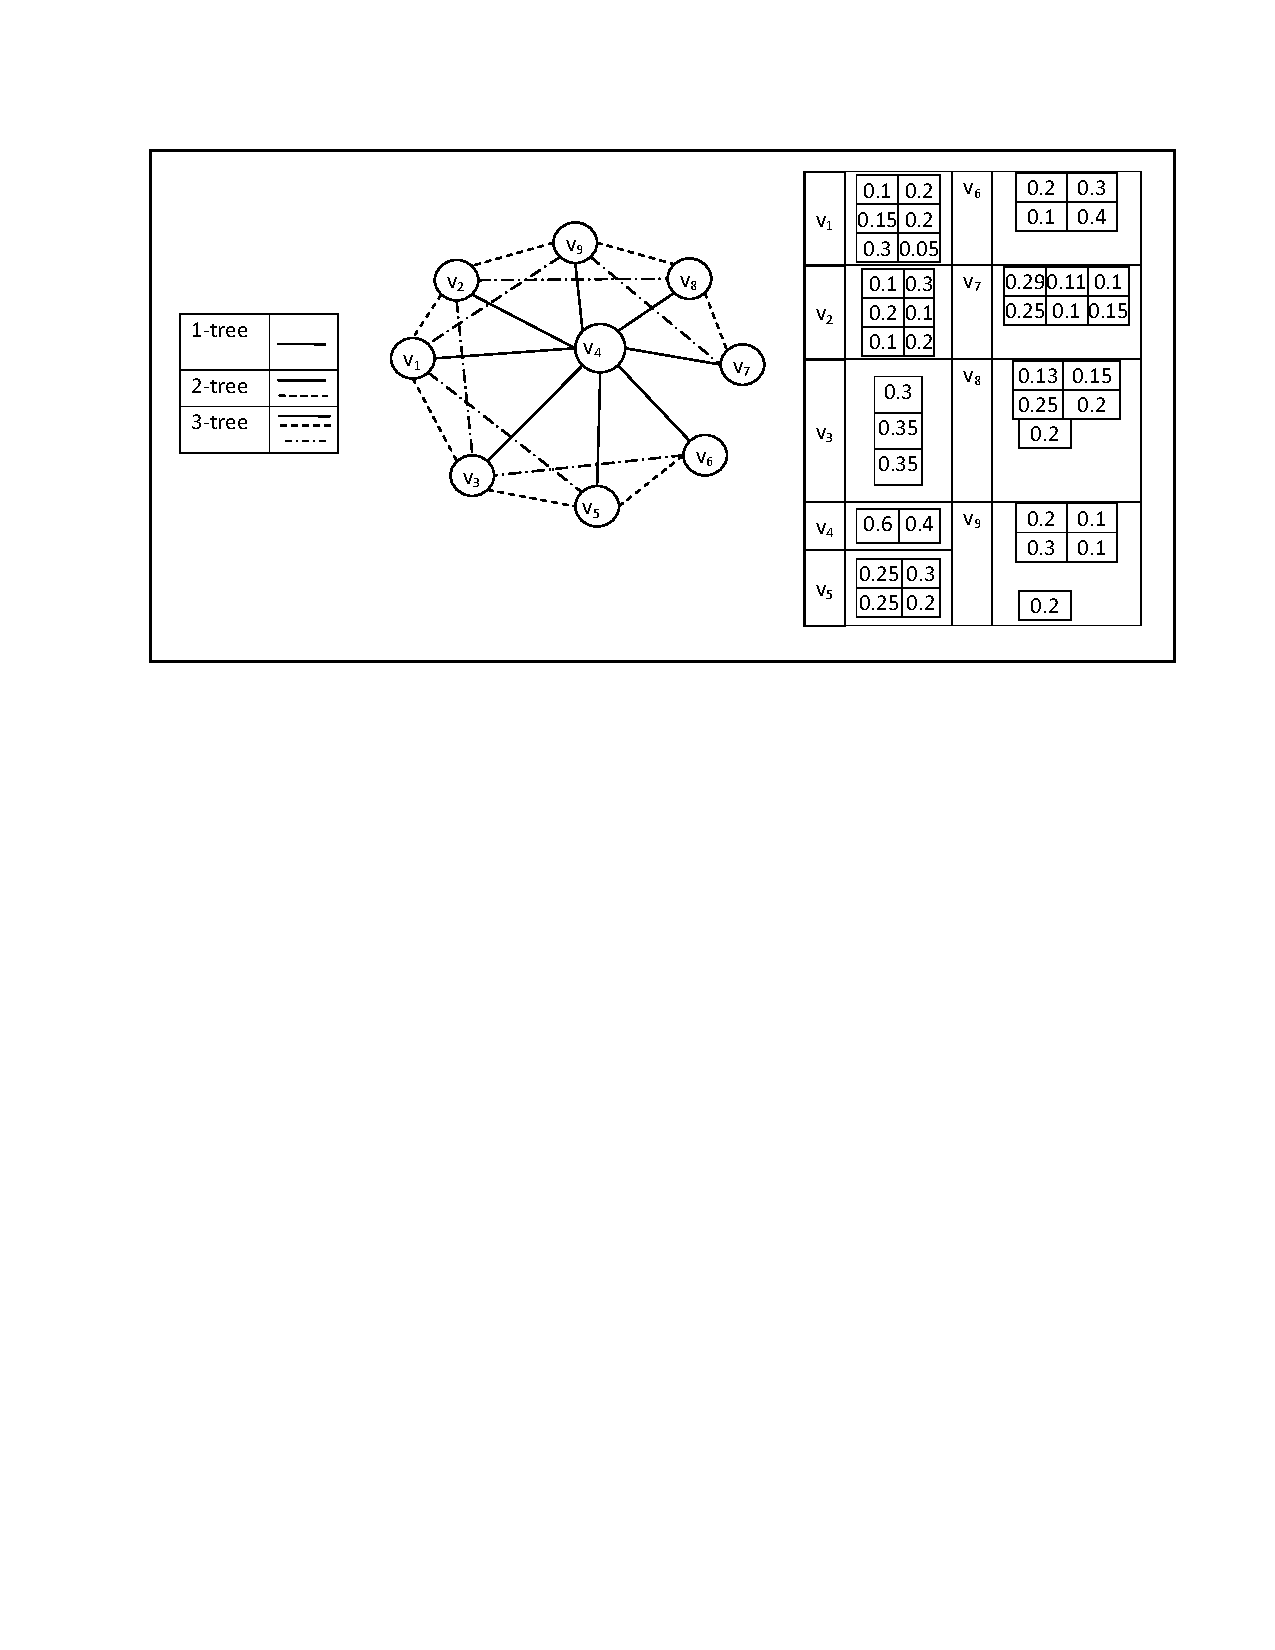
\includegraphics[width=5 in, height=2.5 in]{Example1.pdf}
 \caption{ A UWSN modelled by a $3$-tree.
 \label{fig:3t}
}
\end{figure}
\subsection{Algorithm for $A-CONN$ Problem}
\subsubsection{Key Data-structures}
\label{subsec:kds}
Each clique associated with a table. Each row in the table defines key-value mapping.
\begin{itemize}[noitemsep,nolistsep]
\item A key is a set of sets namely partition(s) of nodes along with corresponding regions in that particular clique. 
\item A value is a probability which is the multiplication of regional probability of nodes for the clique.
\end{itemize}

\begin{exmp}
\normalfont
Fig. \ref{fig:3t} illustrates a graph $G$ which is a $3$-tree with $9$ nodes and their corresponding probabilistic locality set. There are $19$ triangles so there are $19$ cliques associated with this $3$-tree. For each clique the algorithm maintain a table. For every table there are some rows as key-value mapping. For example the clique $<v_1,v_2,v_3>$  can be partitioned $5$ different ways including $\{v_1,v_2,v_3\}, \{v_1,v_2\}\{v_3\}, \{v_1,v_3\}\{v_2\},\{v_1\}\{v_2,v_3\}$ and $\{v_1\}\{v_2\}\{v_3\} $. For each partition there are  $6\times6\times4=144$ rows as key-value mappings because the locality set of node $v_1,v_2$ and $v_3$ are $6,6$ and $4$ respectively. One of the row is ${\{v_1,v_2,v_3\}}^{(1,1,1)} 0.004$ where $v_1,v_2$ and $v_3$ are in same partition with region $1, 1$ and $1$ respectively and the probability $0.004$ is multiplication of corresponding regional probabilities.$\blacksquare$
\end{exmp}
When the algorithm starts elimination node by the order of $PES$ there will be table merging and details is presented in section \ref{sub:Ald}.
\subsubsection{Function Main}
\label{subsub:Main}
We now explain the main steps of function main, merge and merge partitions.
\begin{algorithm} [h]
\Indm
\KwIn{ a UWSN $G=(V,E)$ is a partial $k$-tree where each node, $v\in V$  can be located into a set of regions $R_v=\{r_{(v,1)},r_{(v,2)}...\}$ with probability,    
  $\{p(r_{(v,1)}),p(r_{(v,2)})...\}$ and $(x,y)\in E$ if $x\in V$ can be located one of it's locality set and $y\in V$ can be located one of it's locality set, so that they reach each other. $PES$ is a perfect elimination sequence $(v_1,v_2,...,v_{n-k})$ of $G$.}
\KwOut{ Prob, a solution to the input instance.}
\textbf {Notation:} $Temp$ is a map from keys to probabilities.\\
%\noline
\Indp
\nl \textbf{Initialize } every clique by  a table.\\
\nl\For{$i=1,2,...,n-k$}
{
 \nl node $v_i$ is associated with $k$-cliques, $K_{(v_i,1)},K_{(v_i,2)},..,K_{(v_i,k)}$ \\
 //$T_{(v_i,1)},T_{(v_i,2)},..,T_{(v_i,k)}$ are the tables associated with cliques $K_{(v_i,1)},K_{(v_i,2)},..,K_{(v_i,k)}$ respectively \\
\nl $ Temp=T_{(v_i,1)}$  \\
 \nl \For{$j=2,3..,k$}
 {
  \nl $Temp=merge(Temp,T_{(v_i,j)})$\\
 }
 // clique $K_{(v_i,base)}$ is the base clique and table $T_{(v_i,base)}$ is the base table of node $v_i$
  \nl $Temp=merge(Temp,T_{(v_i,base)})$\\
\nl  \If{$v_i$ is in a partition of $Temp$ by itself}{
\nl ignore the row containing that partition.}

\nl \Else {remove node $v_i$ from $Temp$ and assign the result to $T_{(v_i,base)}$}
}

\nl \Return{Prob=$\sum$(All probability for single partition in the remaining table)}
\caption{Function Main$(G$, $\textbf{R}$, $p(r_{(v,i)})$, $PES )$}
\end{algorithm}



%%Need to writedown main task of this function
Main function eliminates every node according to the PES by merging all cliques associated with that node and updating the result to base clique. The last remaining clique associates with the sink node. Finally  main function calculates the connectivity from the last clique by adding probabilities for those row which is associate with single partition.

In more details, 
\begin{itemize}[noitemsep,nolistsep]
\item   Step $1:$ initialize each clique by a table describe in subsection \ref{subsec:kds}.
\item Step $2:$ processes each node $v_i$ in PES. Every processing node, $v_i$ is associated with $k$ cliques.
\item Step $3:$ finds all those cliques,
 $K_{(v_i,1)},K_{(v_i,2)},..,K_{(v_i,k)}$. 
 \item Step $4:$ assign table $Temp$ with table  $T_{(v_i,1)}$ associated with clique  $K_{(v_i,1)}$.
 \item Steps $5$-$6:$ iteratively merge all associated tables of node $v_i$ and assign the result to table $Temp$ by using $merge$ function. \item Step $7:$ merge $Temp$ table with base table of node $v_i$ $T_{(v_i,base)}$ by using $merge$ function and assign the result to $Temp$. 
 \item Step $8:$ check whether $v_i$ is in a partition by itself i.e. bad set. 
 \item Step $9:$ if there is a bad partition in $Temp$ then the algorithm simply ignore the row along with bad partition.
 \item Step $10:$ remove the vertex $v_i$ and it's locality set from $Temp$ and assign the result to $T_{(v_i,base)}$.
 \item Step $11:$ calculate and return connectivity for the network.
 \end{itemize}
\begin{exmp}
\normalfont
 One of the PES of the $3$-tree depict in fig. \ref{fig:3t} is $<v_1,v_6,v_5,v_7,v_8, v_9>$. In-order to eliminate $v_1$, the algorithm  merge three cliques $<v_1,v_3,v_4>$, $<v_1,v_2,v_3>$ and $<v_1,v_2,v_4>$ to $<v_1,v_2,v_3,v_4>$. Next step the algorithm find the base clique $<v_2,v_3,v_4>$ and merge with  $<v_1,v_2,v_3,v_4>$. Finally it deletes $v_1$  from merged clique and update the result to $<v_2,v_3,v_4> \blacksquare$
\end{exmp}
\begin{table}[!htb]
    %\caption{Global caption}
    \begin{minipage}{.3\linewidth}
      %\caption{$T_1(v_1,v_2,v_3)$}
      \centering
     \begin{tabular}{cc}
\multicolumn{2}{c}{$T_1(v_1,v_2,v_3)$}                           \\ \hline
\multicolumn{1}{|c}{.} & \multicolumn{1}{|c|}{.} \\ \hline
\multicolumn{1}{|l}{$\{v_1,v_2\}^{(1,1)} \{v_3\}^{(2)}$} & \multicolumn{1}{|l|}{$0.002$} \\ \hline
                             \multicolumn{1}{|c}{.} & \multicolumn{1}{|c|}{.} \\ \hline               
                   \multicolumn{1}{|c}{.} & \multicolumn{1}{|c|}{.} \\ \hline
                   \multicolumn{1}{|c}{.} & \multicolumn{1}{|c|}{.} \\ \hline        
\end{tabular}
    \end{minipage}%
    \begin{minipage}{.05\linewidth}

        \begin{tabular}{c}
     $ \times$\\
        \end{tabular}
    \end{minipage}%
     \begin{minipage}{.3\linewidth}
      %\caption{$T_1(v_1,v_2,v_3)$}
      \centering
     \begin{tabular}{cc}
\multicolumn{2}{c}{$T_2(v_1,v_3,v_4)$}                           \\ \hline
\multicolumn{1}{|c}{.} & \multicolumn{1}{|c|}{.} \\ \hline
\multicolumn{1}{|l}{$\{v_1\}^{(1)}\{v_3,v_4\}^{(2,1)}$} & \multicolumn{1}{|l|}{$0.008$} \\ \hline
                   \multicolumn{1}{|c}{.} & \multicolumn{1}{|c|}{.} \\ \hline               
                   \multicolumn{1}{|c}{.} & \multicolumn{1}{|c|}{.} \\ \hline
                   \multicolumn{1}{|c}{.} & \multicolumn{1}{|c|}{.} \\ \hline        
\end{tabular}
    \end{minipage}%
      \begin{minipage}{.06\linewidth}

        \begin{tabular}{c}
     $ \Rightarrow$\\
        \end{tabular}
    \end{minipage}%
     \begin{minipage}{.3\linewidth}
      %\caption{$T_1(v_1,v_2,v_3)$}
      \centering
     \begin{tabular}{cc}
\multicolumn{2}{c}{$Temp(v_1,v_2,v_3,v_4)$}                           \\ \hline
\multicolumn{1}{|c}{.} & \multicolumn{1}{|c|}{.} \\ \hline
  \multicolumn{1}{|l}{$\{v_1,v_2\}^{(1,1)}\{v_3,v_4\}^{(2,1)}$} & \multicolumn{1}{|l|}{$0.0008$} \\ \hline         
                   \multicolumn{1}{|c}{.} & \multicolumn{1}{|c|}{.} \\ \hline                 
                   \multicolumn{1}{|c}{.} & \multicolumn{1}{|c|}{.} \\ \hline
                   \multicolumn{1}{|c}{.} & \multicolumn{1}{|c|}{.} \\ \hline        
\end{tabular}
    \end{minipage}\\
    \begin{minipage}{1.0\linewidth}
       \centering
 
        \begin{tabular}{c}
Figure 3 a). Merging two table into $Temp$
        \end{tabular}
    \end{minipage}\\
     \begin{minipage}{.4\linewidth}
      %\caption{$T_1(v_1,v_2,v_3)$}
      \centering
     \begin{tabular}{cc}
\multicolumn{2}{c}{$Temp(v_1,v_2,v_3,v_4)$}                           \\ \hline
\multicolumn{1}{|c}{.} & \multicolumn{1}{|c|}{.} \\ \hline
  \multicolumn{1}{|l}{$\{v_1,v_2\}^{(1,1)}\{v_3,v_4\}^{(2,1)}$} & \multicolumn{1}{|l|}{$0.0008$} \\ \hline         
                   \multicolumn{1}{|c}{.} & \multicolumn{1}{|c|}{.} \\ \hline                 
                   \multicolumn{1}{|c}{.} & \multicolumn{1}{|c|}{.} \\ \hline
                   \multicolumn{1}{|c}{.} & \multicolumn{1}{|c|}{.} \\ \hline        
\end{tabular}
    \end{minipage}%
     \begin{minipage}{.06\linewidth}
     
        \begin{tabular}{c}
     $ \Rightarrow$\\
        \end{tabular}
    \end{minipage}%
    \begin{minipage}{.3\linewidth}
      %\caption{$T_1(v_1,v_2,v_3)$}
      \centering
     \begin{tabular}{cc}
\multicolumn{2}{c}{$Temp(v_2,v_3,v_4)$}                           \\ \hline
\multicolumn{1}{|c}{.} & \multicolumn{1}{|c|}{.} \\ \hline
  \multicolumn{1}{|l}{$\{v_2\}^{(1)}\{v_3,v_4\}^{(2,1)}$} & \multicolumn{1}{|l|}{$0.0008$} \\ \hline         
                   \multicolumn{1}{|c}{.} & \multicolumn{1}{|c|}{.} \\ \hline                 
                   \multicolumn{1}{|c}{.} & \multicolumn{1}{|c|}{.} \\ \hline
                   \multicolumn{1}{|c}{.} & \multicolumn{1}{|c|}{.} \\ \hline        
\end{tabular}
    \end{minipage}\\
      \begin{minipage}{1.0\linewidth}
       \centering

        \begin{tabular}{c}
Figure 3 b). Deleting node $v_1$ from $Temp$
        \end{tabular}
    \end{minipage}\\
\end{table}
\subsubsection{Function Merge}
\label{subsub:Mrg}
The primary task of merge function is to merge two table $T_1, T_2$, update keys and values of the newly created table $T$ and return the table $T$.

In more details, 
\begin{itemize}[noitemsep,nolistsep]
\item Step $1:$ finds the common vertices between two tables  and assign the common nodes probability $1$.
\item Step $2:$  check if whether or not the common vertex set $C$ is empty. If it is empty then the algorithm returns otherwise go to next step. 
\item Steps $3$-$5:$  performs the row-wise merging by using function $mpar$ and create another row.
\item  Steps $6$-$7:$ updates the locality set for every vertex $v$ of newly created row. 
\item Steps $8$-$9:$ calculates the regional probability of common nodes. 
\item Step $10:$ updates the newly created row probability by multiplying row-wise probability and dividing by the sum of common nodes regional probabilities. 
\item Step $11:$ insert the row into table $T$ and 
\item Step $12:$ return table $T$.
\end{itemize}
\begin{exmp}
\normalfont
Fig 3 a). illustrates merging row  $\{v_1,v_2\}^{\{1,1\}}\{v_3\}^{\{2\}}$ $0.002$ of table $T_1$ with row $\{v_1\}^{\{1\}}\{v_3,v_4\}^{\{2,1\}}$ $0.008$ of table $T_2$ which is fundamental operation for merging two tables. The function merge uses $pMerge$ function which takes two partitions $\{v_1,v_2\}\{v_3\}$ and $\{v_1\}\{v_3,v_4\}$ and returned $\{v_1,v_2\}\{v_3,v_4\}$ because $\{v_1,v_2\}\cup \{v_1\}=\{v_1,v_2\}$ and $\{v_3\}\cup \{v_3,v_4\}=\{v_3,v_4\}$. The merge function updates the locality set of each node of the merged partition $\{v_1,v_2\}^{\{1,1\}}\{v_3,v_4\}^{\{2,1\}}$ from the locality set of nodes in merging partitions. There are two common nodes $v_1$ and $v_3$ located in region $1$ and $2$ respectively with probability $0.1$ and $0.2$ respectively in the merging partitions. It update the probability of newly created partition $0.0008$ by multiplying row-wise probabilities $0.002\times 0.008$ and dividing the probability by product of the common nodes corresponding regional probabilities $0.1\times 0.2$.

Fig 3 b). shows the deletion of node $v_1$ from $Temp$. The function main simply look for the node and remove it and it's locality set from key.$\blacksquare$
\end{exmp}
\begin{algorithm}[H]
\Indm  
\KwIn{ Two tables $T_1$ and $T_2$ that share at least one common vertex}
\KwOut{A  table $T$}

\textbf{Notation} $C$ is a set of vertices and $Obj$ is a row of table $T$ and $Prob\_C$ is a double variable\\
\Indp
\nl \textbf{set} $C=$ the set of common vertices between $T_1$ and $T_2$ , set $Prob\_C=1$\\
 \nl \If{$C\neq \emptyset$}{
 \nl \ForEach{row $r$ in $T_1$}
 {
 \nl \ForEach{row $s$ in $T_2$}
 {
  \nl  $Obj.par=$pMerge($r.par$,$s.par$)\\
   \nl \ForEach{vertex $v_i$ in $Obj.par$ where $i=1,2,..,k+1$}
    {
   \nl $Obj.loc[v_i]=r.loc[v_i]||s.loc[v_i]$\\
    }
    
   \nl \ForEach{vertex  $v\in C$}
    {
   \nl $Prob\_C=Prob\_C*s.loc[v]$
    }
\nl $ Obj<Obj.par:Obj.loc>=\frac{Prob[r]\times Prob[s]}{Prob\_C}$\\
\nl Insert $Obj$ in $T$ as a row.\\
}
  }
  }
\nl \Return {Table T}

 \caption{Function merge($T_1,T_2$)}
\end{algorithm}

\subsubsection{Function Merge Partitions }
\label{subsub:fMpar}
 The merging partitions is mainly done using the union operation by mapr function. The mpar function takes as input two partitions $P_1$, $P_2$ and merge them into one partition $P$.

In more details,  
\begin{itemize}[noitemsep,nolistsep]
\item Steps $1$-$2:$ adds all the sets of $P_2$ to $P_1$.
\item Steps $3$-$4:$ selects two sets $s^*$ and $t^*$ from partition $P_1$ 
\item Step $5$: checks whether or not they are disjoint . If they are  not disjoint then it will go to step 6 otherwise it will return to step 4.
\item Step $6:$ delete $s^*$ from $P_1$.
\item Step $7:$ computes the union of $s^*$ and $t^*$ and insert it at the beginning of partition $P_1$.
\item Step $8:$ delete $t^*$ from $P_1$.
\item Steps $9$-$10:$ set the iterator to the beginning of $P_1$ and return to step 5.
\item Step $11:$ assign $P_1$ to $P$ and finally the algorithm return $P$.
\end{itemize}


\begin{algorithm}[H]
\KwIn{Two partitions $P_1$ and $P_2$}
\KwOut{A partition $P$}
\textbf{Notation:} $s$ and $t$ are two set iterators and their corresponding set are indicated by $s^*$ and $t^*$.\\ 
\nl \ForEach{ set $s^*$ in $P_2$}
{
\nl $P_1.push\_back(s^*)$
}
\nl \For{ $(s=P_1.begin()$; $s \neq P_1.end()$;  $++s)$}
{
\nl \For{ $(t=s.next()$; $t \neq P_1.end()$; $++t)$}
{
 \nl \If{$s^*\cap t^* \neq \emptyset$}
  {
\nl  	$  P_1.push\_front(s^*\cup t^*$) \\
\nl$P_1.delete(s^*)$\\
  \nl $P_1.delete(t^*)$\\
  \nl $s=P_1.begin()$\\
   \nl$break$\\
  }
}
}
\nl set $P=P_1$\\
\Return{P}
\caption{function pMerge($P_1$, $P_2$)}
\end{algorithm}






\subsection{Verification Cases}
\label{subsec:vc}
In this subsection we are going to present some cases by using these one can verify the correctness of our algorithm.
\begin{figure}

\begin{minipage}{.9\linewidth}
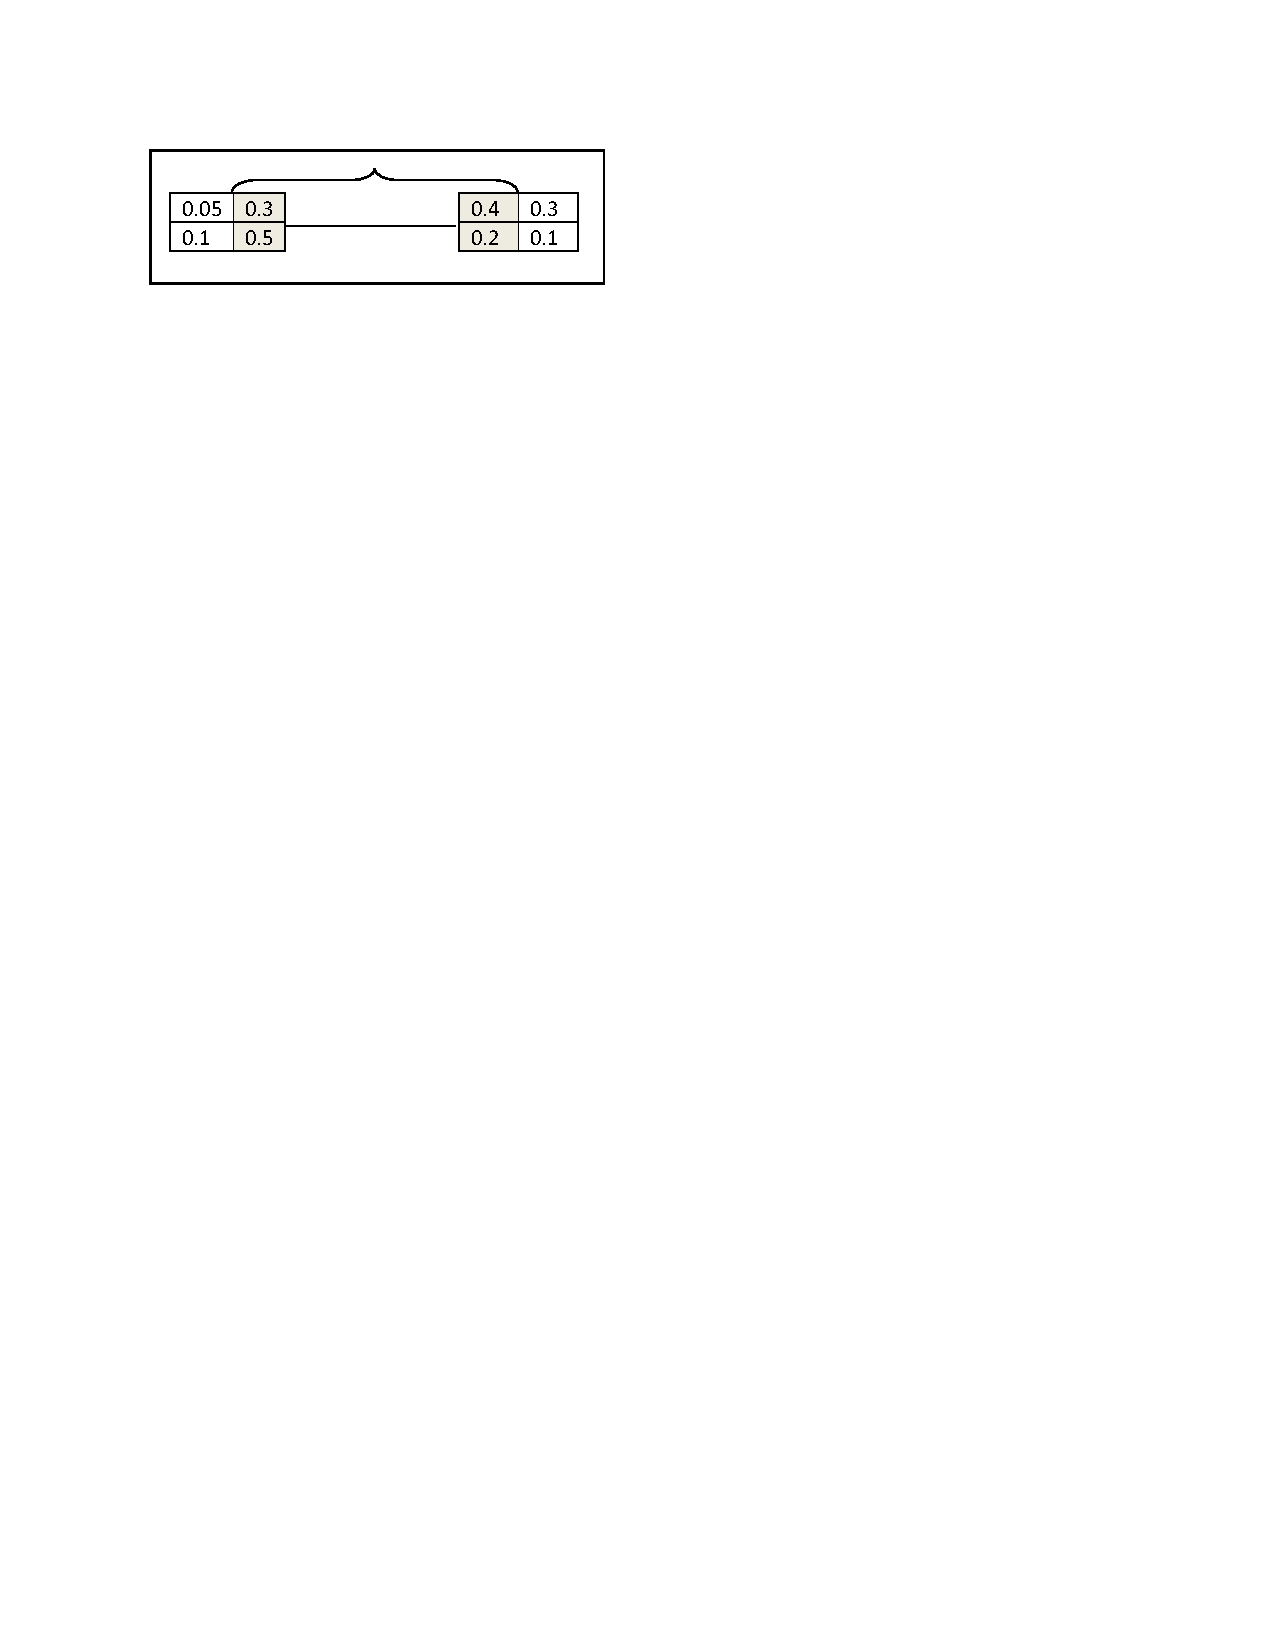
\includegraphics[width=3 in, height=.6 in]{verification.pdf}
\caption{A simple tree with 2 nodes}
\end{minipage}
\label{fig:var}
\end{figure}
\begin{itemize}
\item For a partial $k$-tree, there should be more than one PES. In our algorithm, we tried all elimination sequence and we got same result.
\item The algorithm exhaustively consider all possible configuration to calculate the connectivity. Consider a small example with two nodes illustrates in fig \ref{fig:var} where $v_1$ and $v_2$ has the locality set of four for both nodes. In-order to find connectivity the algorithm consider all possible configuration and there are $16$ possible configurations. But $v_1$ can reach node $v_2$ when $v_1$ is in regions with probability $0.3$ and $0.5$ and $v_2$ is in regions with probability $0.4$ and $0.2$. So the connectivity for this small network is $0.8 \times 0.6=0.48$.

\end{itemize}

\subsection{Correctness}
In this section we prove the correctness of our algorithm. It is an exhaustive algorithm which takes care all possible configuration.
Our algorithm consists of two fundamental operation, partition merge and table merge. First we prove that partition merge and table merge are correct then we prove that our algorithm is correct.\\
 The partition merge perform core operations of the algorithm. The partition merge is correct because it is merging two partitions into one given that they share at least one node. The table merge is correct because of the following reason. The table merge is merging each row of one table with each row of another table by holding the condition that they share atleast one node with same regional position. It is using partition merge in-order to merge two rows which is correct. The main algorithm is elimination a node by merging all clique associated with that node and updating the merged clique with base clique of that node. Each clique is associated with table so cliques are merged by using table merge operation which is correct. That concludes that the algorithm is correct.
\subsection{Running time}
\begin{itemize}[noitemsep]
\item The number of nodes in a table for $k$-tree $=k$.
\item The number of ways $k$ nodes can be partitioned $=2^k$.
\item locality set of a node which is largest in comparison with other nodes $=l_{max}$.
\item The number of ways each partition reappear $=l_{max}^k$.
\item So the length of a table $=l_{max}^k \times 2^k$.
\item In-order to merge two tables total number of operation$=(l_{max}^k \times 2^k)^2$.
\item When we are elimination a node the number of clique associated with a node for $k$-tree$=k$ and there is one base clique associated with every clique. So total number of clique associated with a node $=k+1$.
\item Total number of operation to eliminate one node $=(l_{max}^k \times 2^k)^{k+1}$
\item Total number of node we are eliminating $=N$.
\item So the total cost $=N \times( l_{max}^k \times 2^k)^{k+1}$
\
\end{itemize}
\subsection{Simulation Results}
In this section we present simulation results that aim to investigate the following aspect 
\begin{itemize}
\item[(a)] complexity of our algorithm increases with increasing the value of $k$ for partial $k$-tree.
\item[(b)] influence of $k$ on accuracy where $k=1,2,3,..$.
\item[(c)] effect of choosing different $k$-trees.
\end{itemize}
 
\begin{table}[!htb]
    %\caption{Global caption}
    \begin{minipage}{.5\linewidth}
    \caption{Running time (RT) with respect to $k$}
      \centering
     \begin{tabular}{|c|c|c|c|}
     \hline
         k& Network I & Network II & Network III \\
     \hline
     1&30& 30& 20 \\\hline
     2&290 &380&380	\\\hline
3 &85000&875000&940000	 \\\hline
 



\end{tabular}
    \end{minipage}
    \begin{minipage}{.5\linewidth}
      \caption{Accuracy with respect to $k$}
      \centering
     \begin{tabular}{|c|c|c|c|}
     \hline
     k& Network I & Network II & Network III \\
     \hline
      1 & 62&32.96& 81.8 \\\hline
2 &71.2 & 36.15& 98.95\\\hline
3 &75& 37.31& 100\\\hline
\end{tabular}
    \end{minipage}\\
   % \caption{Running time(RT) and accuracy increases with respect to $k$}
    
\end{table}
\begin{figure}
\begin{minipage}{.9\linewidth}
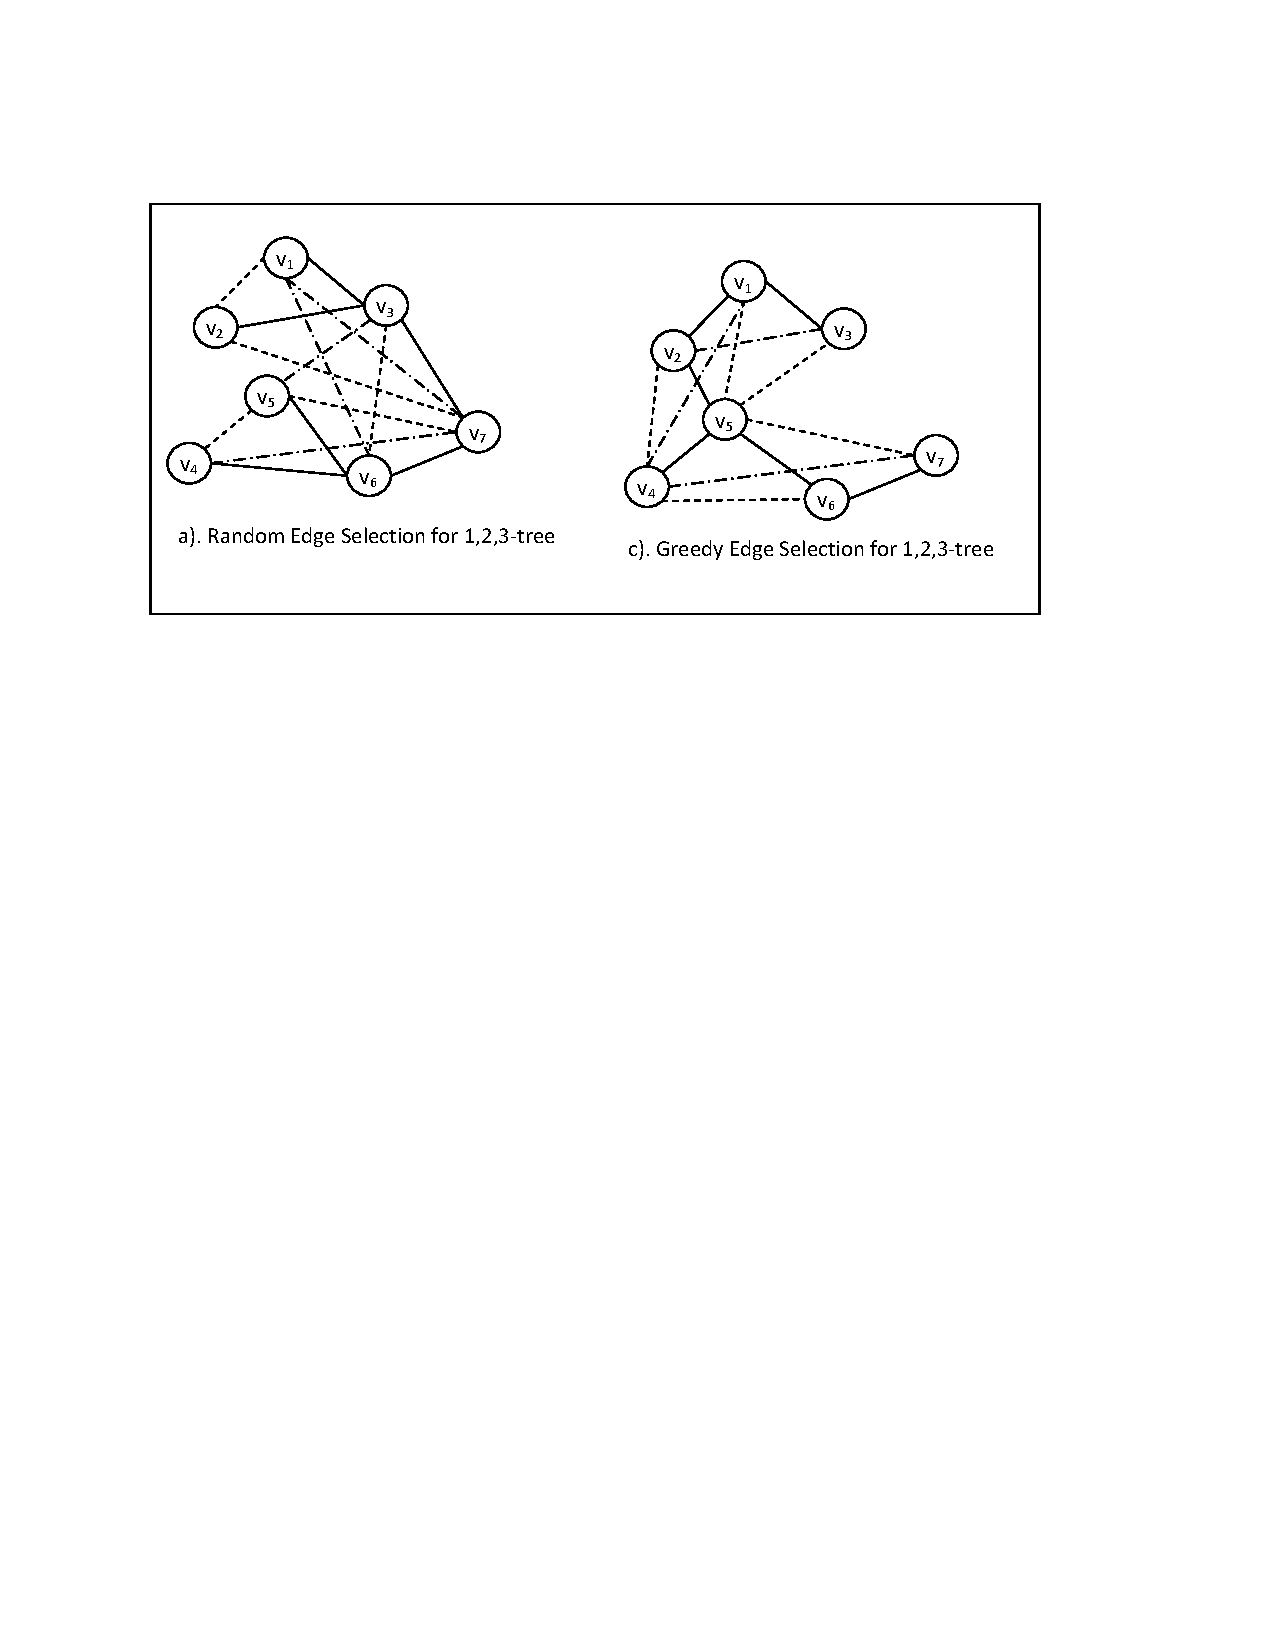
\includegraphics[width=6 in, height=2.8 in]{Edge_selection1.pdf}
\caption{Greedy Vs Random Edge selection}
\label{Fig:ES}
\end{minipage}
\end{figure}


\begin{figure}
\begin{minipage}{.9\linewidth}
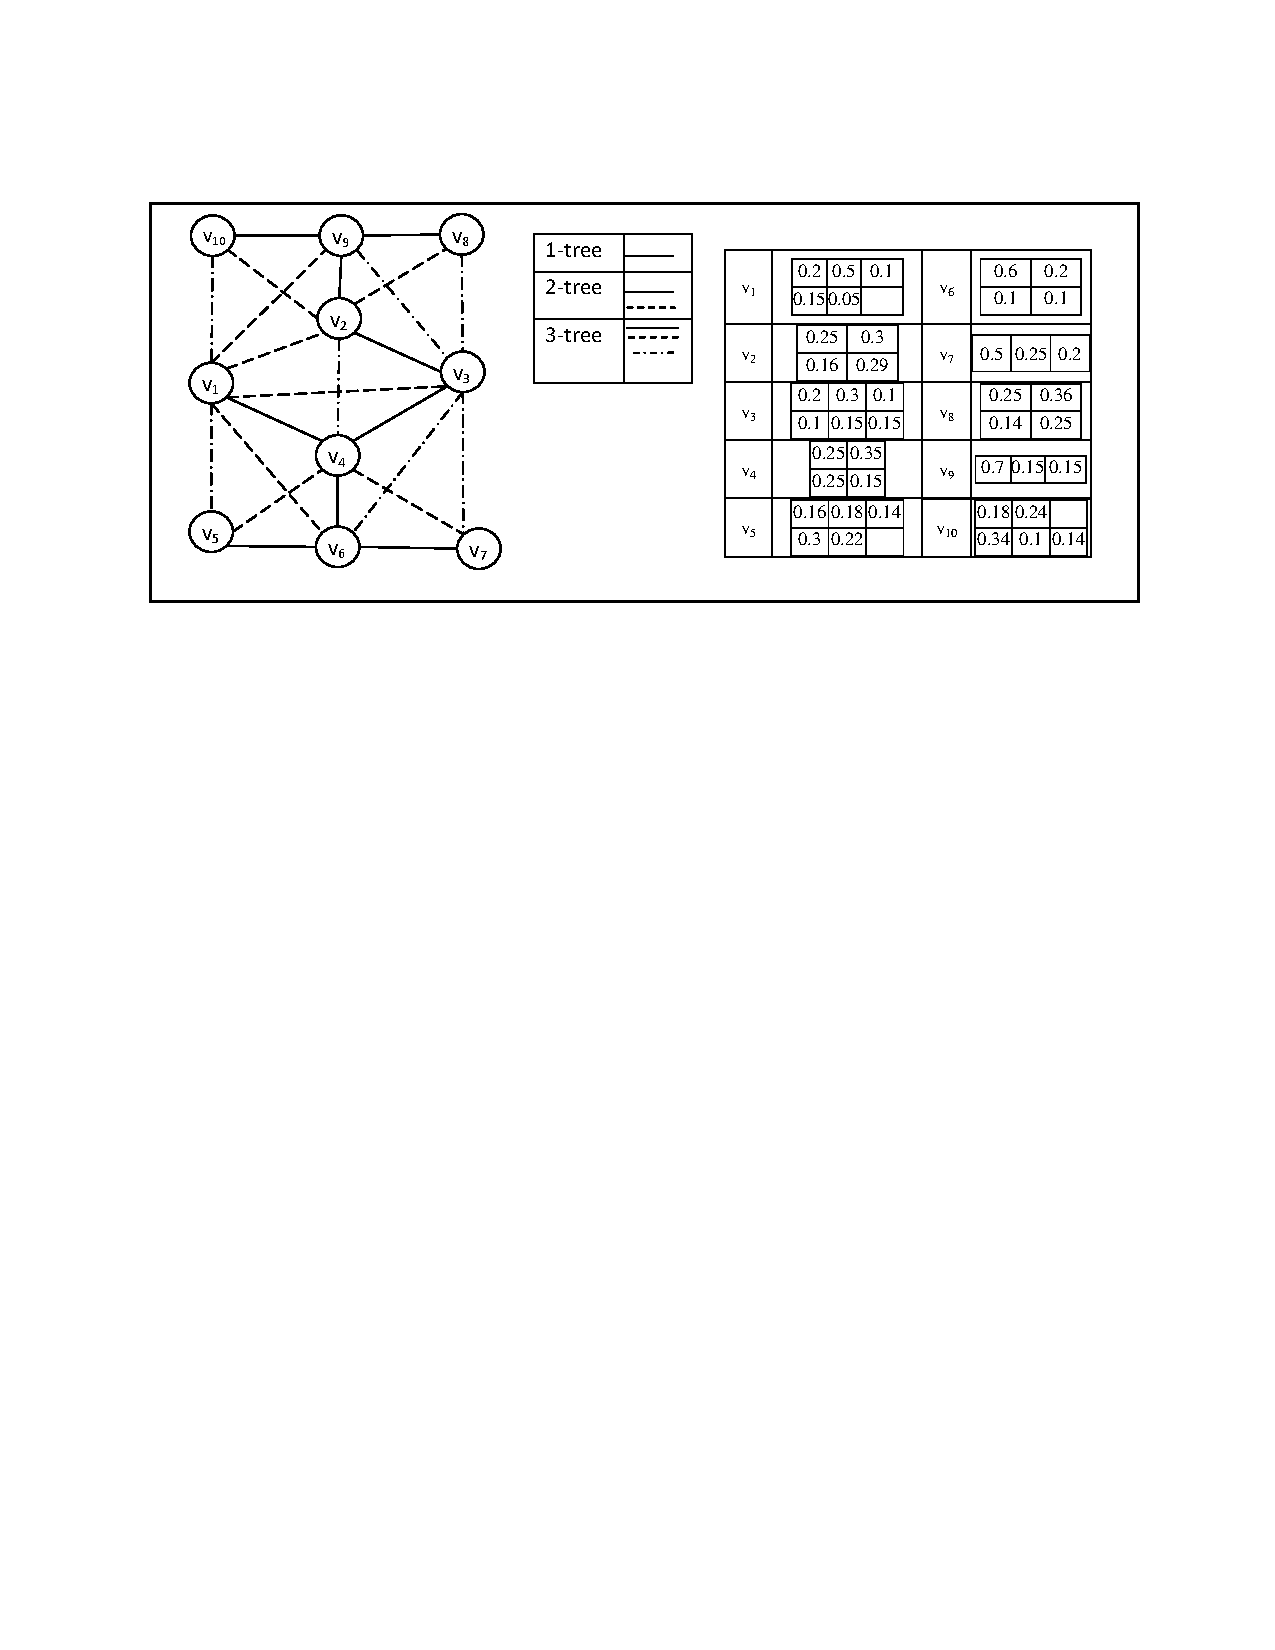
\includegraphics[width=6 in, height=2.8 in]{netI.pdf}
\caption{NetworkI}
\end{minipage}
\begin{minipage}{.9\linewidth}
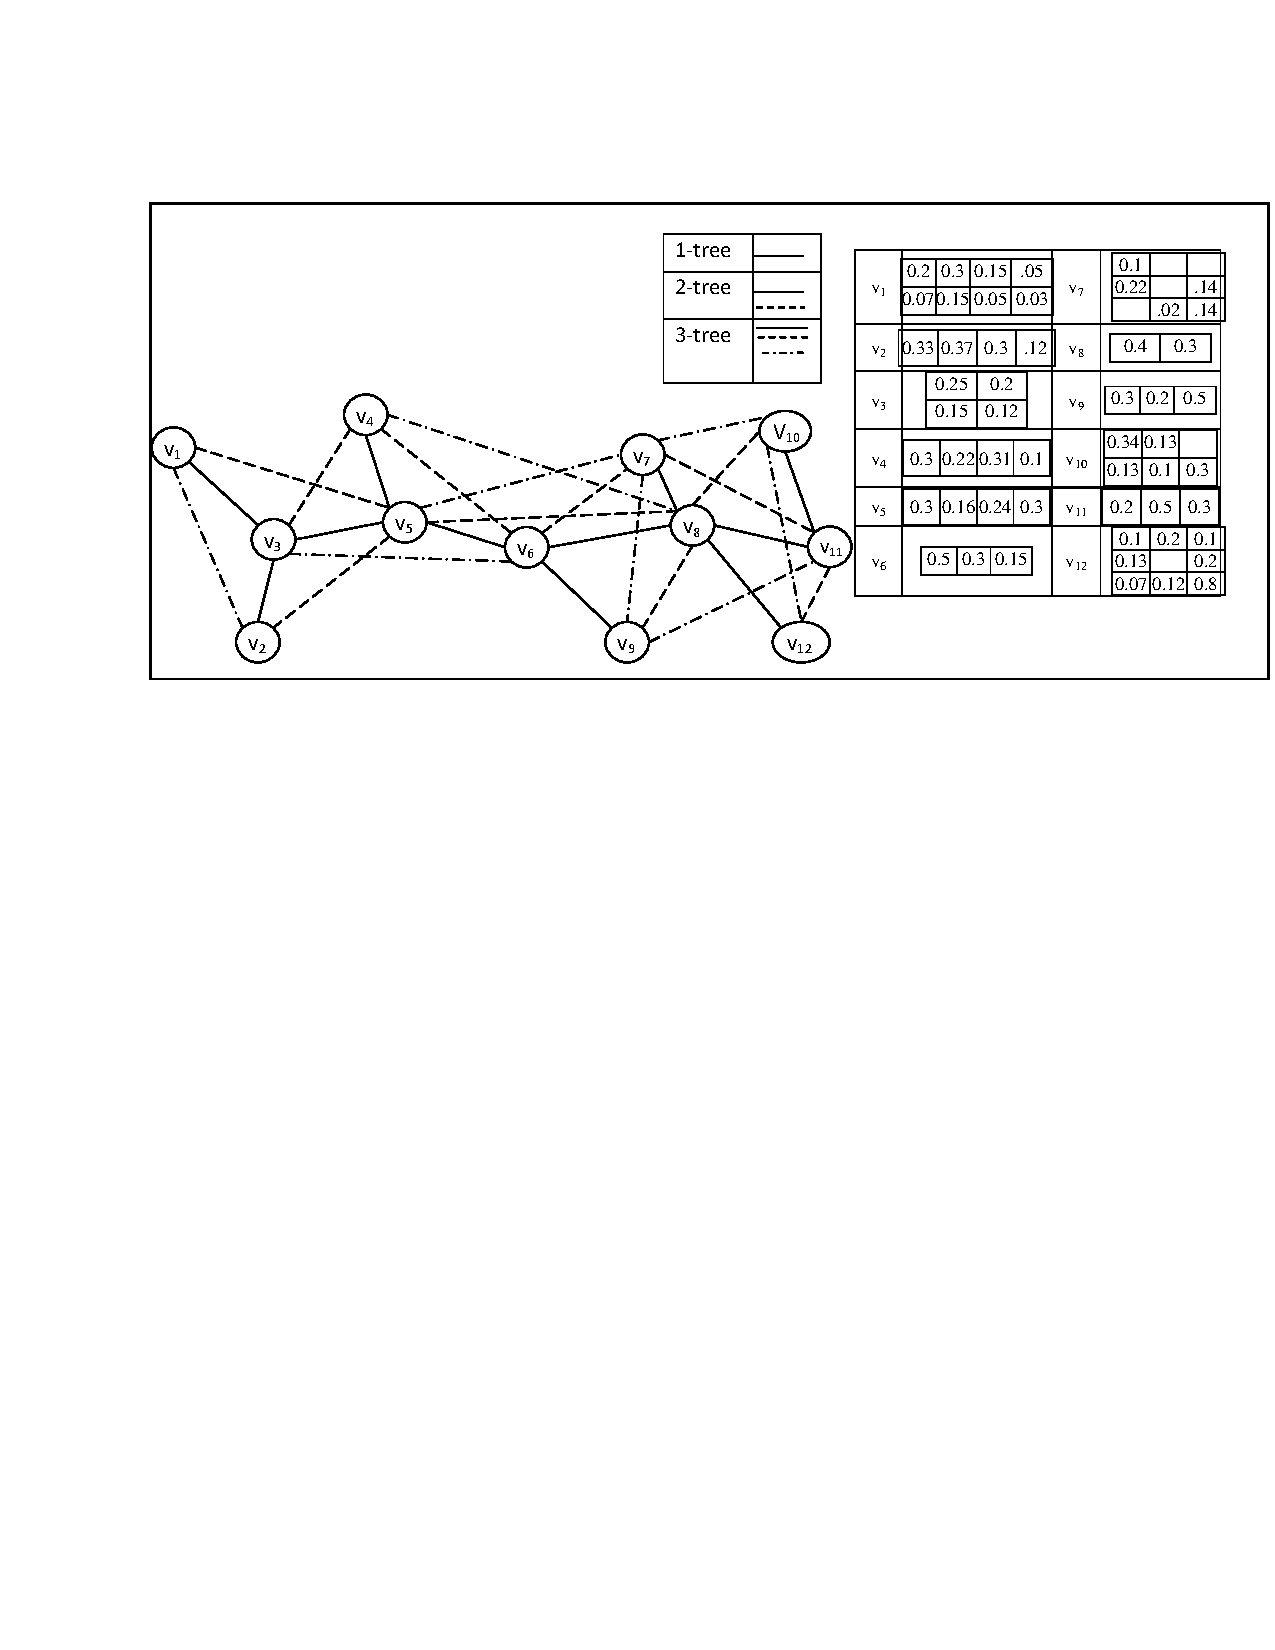
\includegraphics[width=6 in, height=2.7 in]{NetworkII.pdf}
\caption{NetworkII}
\end{minipage}
\begin{minipage}{.9\linewidth}
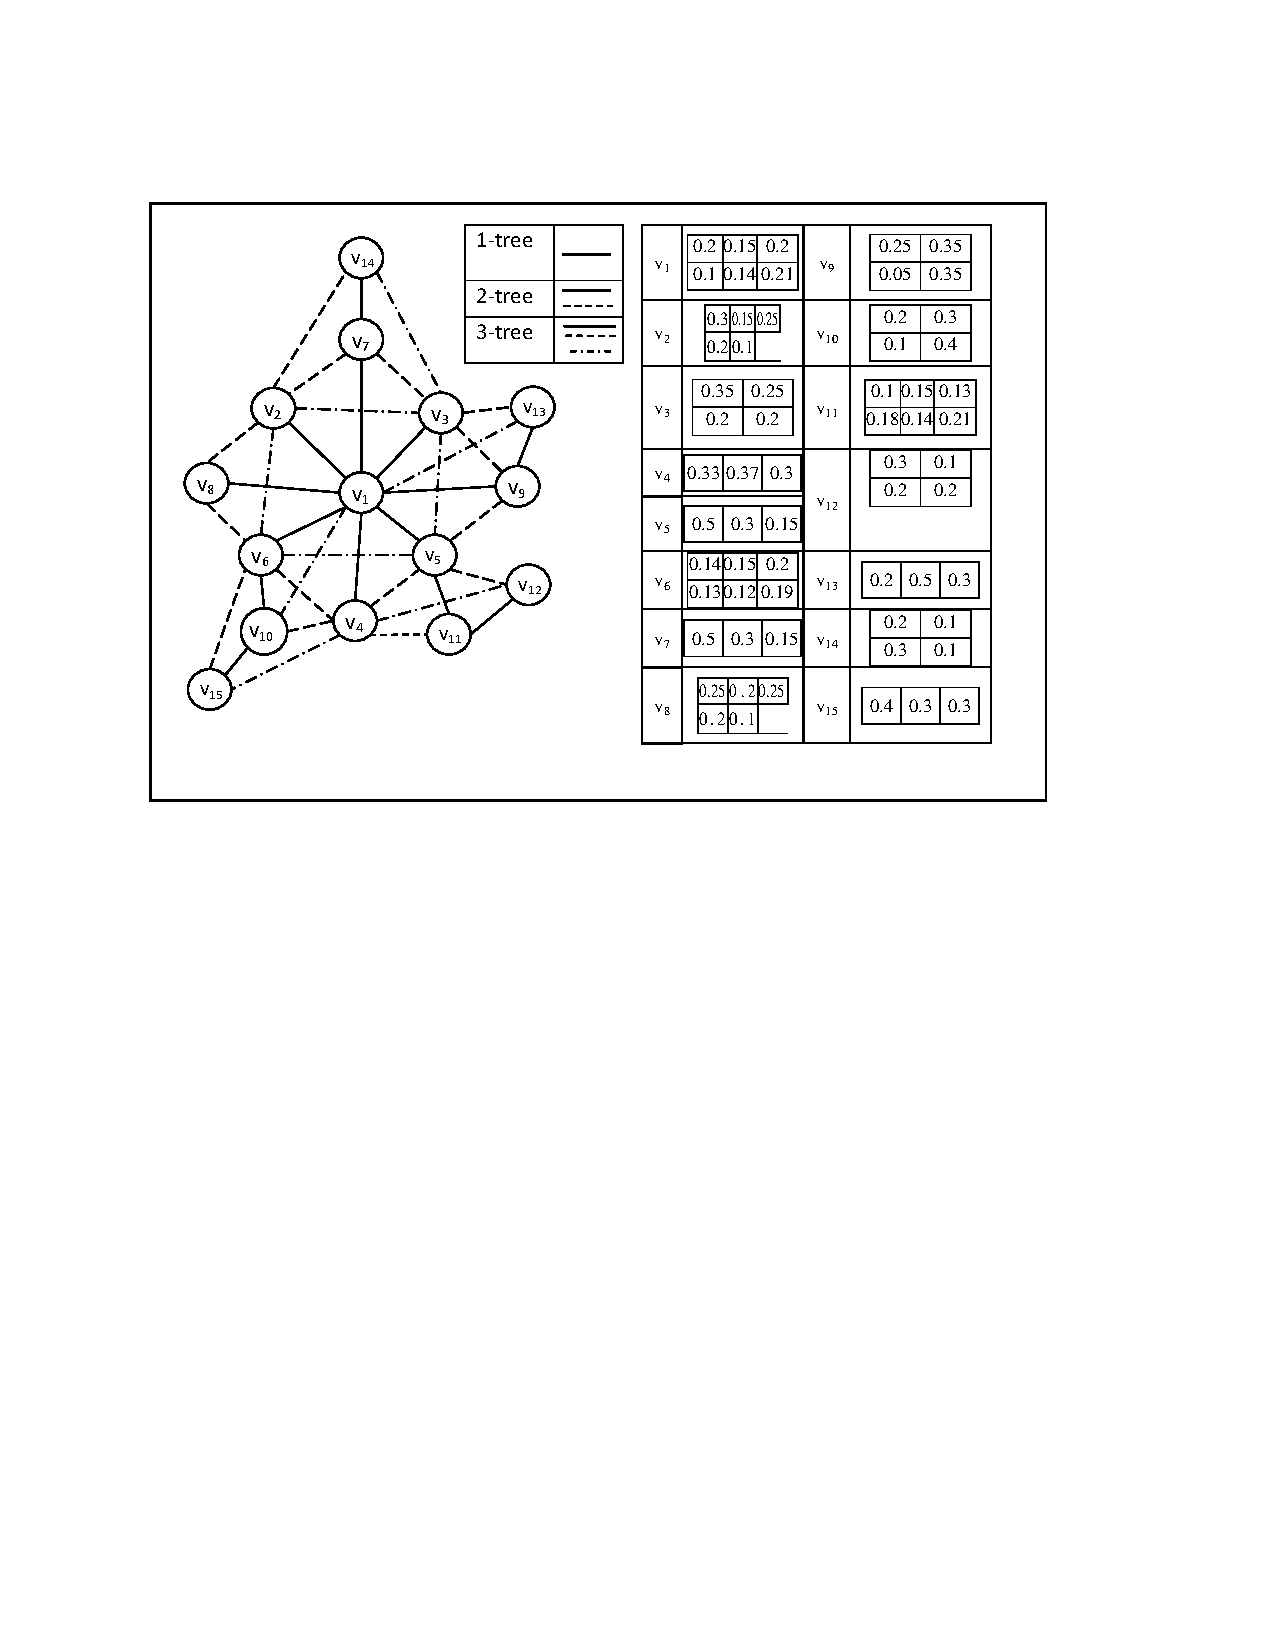
\includegraphics[width=6 in, height=2.6 in]{NetworkIII.pdf}
\caption{NetworkIII}
\end{minipage}
\label{fig:NTRK}
\end{figure}
We used three networks in-order represent running time and accuracy. Network I consists of $7$ nodes with locality set of each node range from $4$ to $8$. Network II consists of $9$ nodes where each node can be located from $3$ to $6$ locations.Network III consists of $12$ nodes with locality set of each node range from $2$ to $8$.
\begin{figure}
\begin{minipage}[]{.5\linewidth}
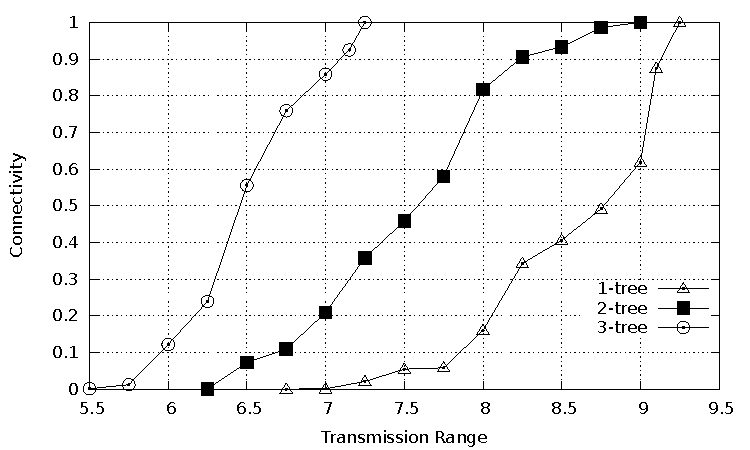
\includegraphics[width=3 in, height=2.5 in]{random.pdf}
 \caption{ Connectivity versus transmission range with  random edge selection.
}
\label{fig:res}
\end{minipage}
\begin{minipage}{.5\linewidth}
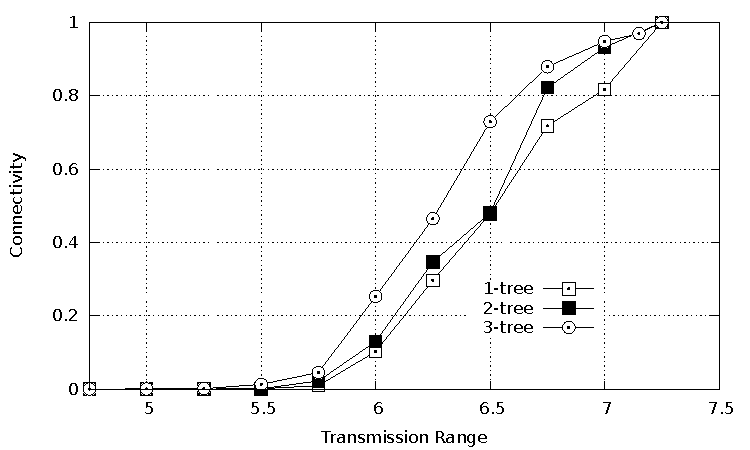
\includegraphics[width=3 in, height=2.5 in]{Greedy.pdf}
 \caption{ Connectivity versus transmission range with greedy edge selection.
}
\label{fig:ges}
 \end{minipage}
\end{figure}
\begin{itemize}
\item[a)] \textbf{$k$ versus running time} table 1 shows three scenarios running time with respect to $k$ of. In every scenario the running time of the algorithm increases with $k$. We also observe that difference between the running time $1$-tree and $2$-tree are $10$ to $15$ times where the running time between $2$-tree and $3$-tree are more than $1000$ times. This is because of complexity of $3$-tree is much more than $2$-tree.\\
\item [b)]\textbf{$k$ versus accuracy}
table 2 illustrates accuracy increases with $k$. The increase of accuracy is large for $1$-tree to $2$-tree than for $2$-tree to $3$-tree. 

\item [c1)] \textbf{Effect of random edge selection.} Fig \ref{fig:res} illustrates connectivity versus transmission range when the algorithm selects randomly. We have the following observation from fig \ref{fig:res}.

 
\begin{itemize}[noitemsep,nolistsep]
\item with increase of transmission range the connectivity is also increasing. This is due to,increase of transmission range the probability of an edge between two nodes also increasing.
\item connectivity for $2$-tree is always greater than or equal to the connectivity of $1$-tree for same transmission range. This is because in $2$-tree there are more edges in comparison with $1$-tree.
\item The above is also true for $2$-tree to $3$-tree.
\end{itemize}
\item [c2)]\textbf{Effect of greedy edge selection.} Fig \ref{fig:ges} illustrates connectivity versus transmission range when we are selecting edges by greedy techniques. In greedy techniques those edges are selected which has a high probable values. Fig \ref{Fig:ES} illustrates greedy edge selection vs random edge selection scenario.  It is observable from figure that the network is fully connected with a smaller transmission range for all tree in comparison with random edge selection strategy.
\end{itemize}
\subsection{Summary}
\section{$A-CONN$ with Relays Problem}
\subsection{Introduction}
In this section we add relay nodes to our network. So our data structures changes as a result main algorithm and merge function also changes in some aspect. We describe the updates and show the results after adding relays.\\
We added relays, $Rel\subset V$ to the network in addition to sensor nodes which is referring target $Tar\subset V$ node in this section.
\begin{figure}[h]

\centering
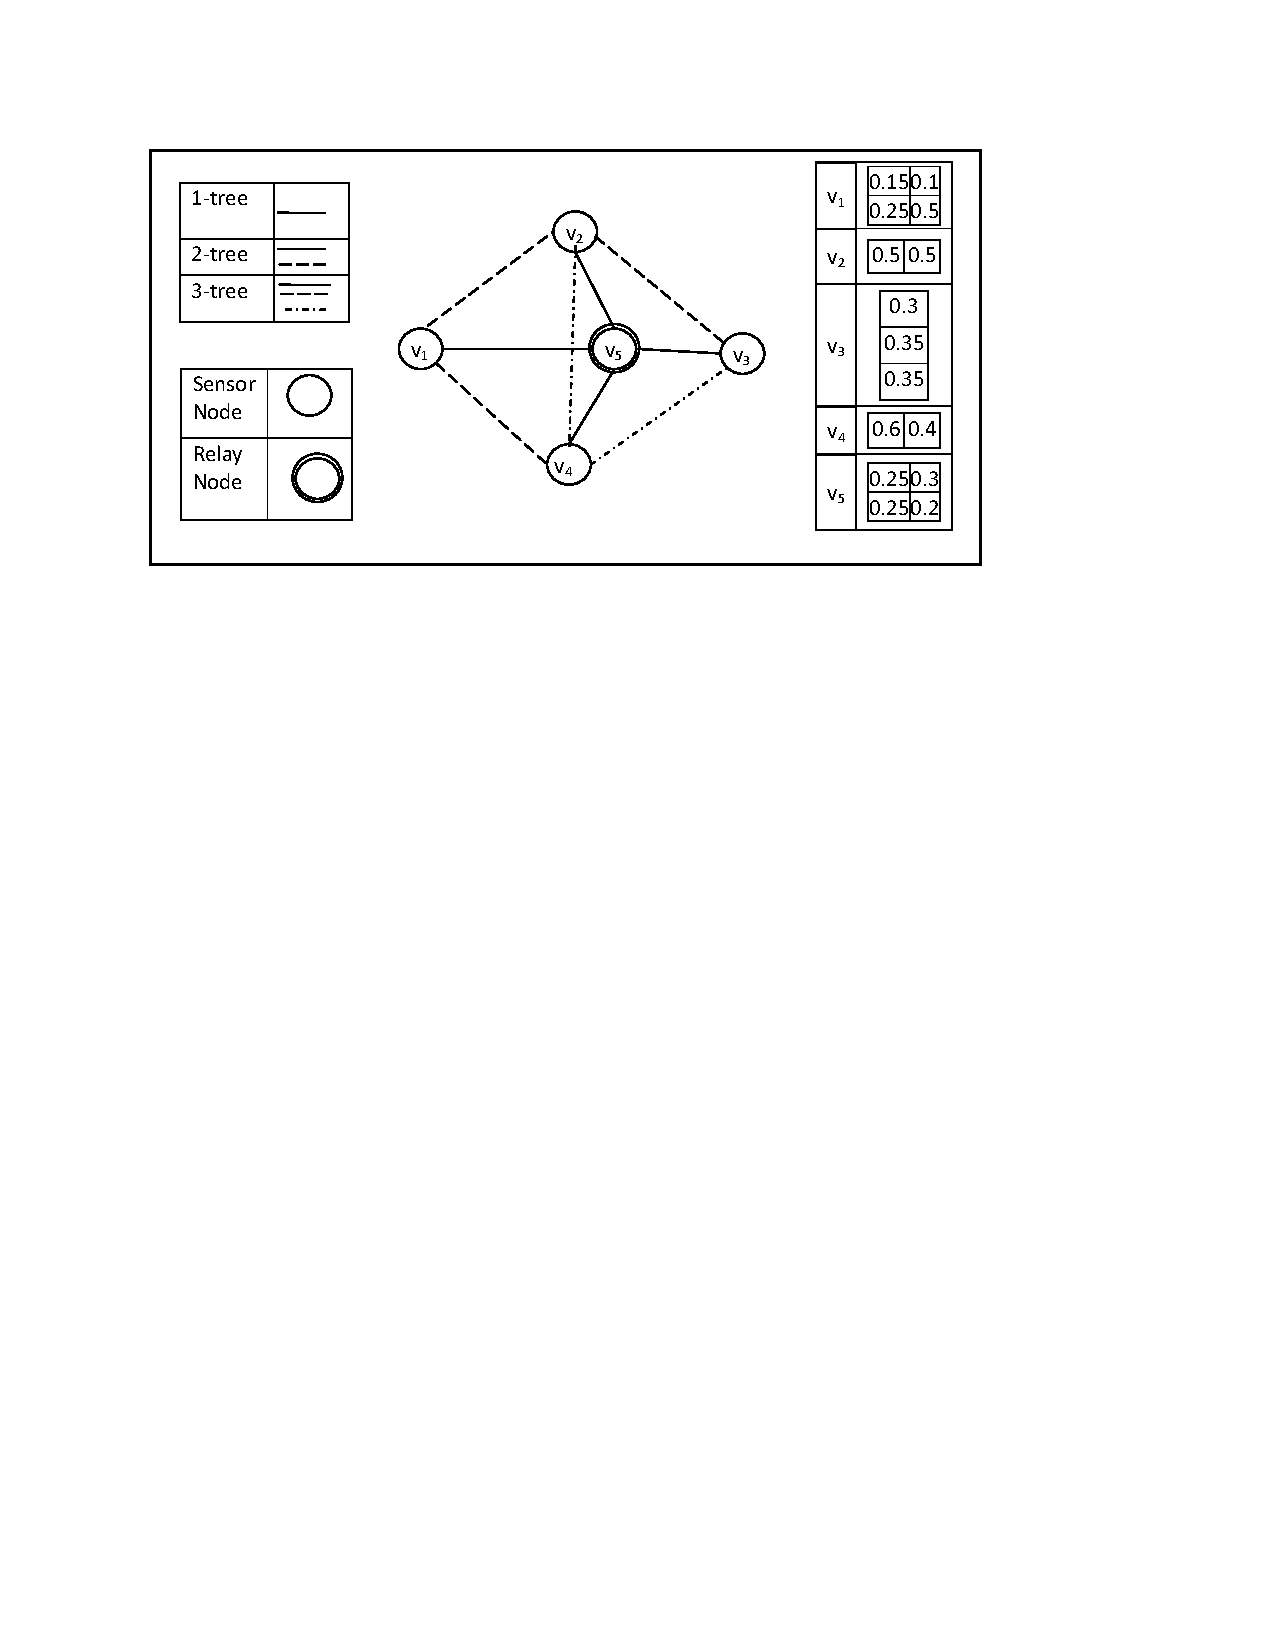
\includegraphics[width=6 in, height=2.5 in]{Relay.pdf}
 \caption{A partial \(2\)-tree with \(6\) nodes.
}
\label{fig:relay1}
\end{figure}
\begin{exmp}
\normalfont
Fig \ref{fig:relay1} illustrates a network of 6 nodes where $v_1,v_2,v_3$ and $v_4$ are target nodes and $v_5, v_6$ are relays. $v_5$ is enhancing the connectivity of the network but $v_6$ is not  increasing the connectivity. So we can simply ignore $v_6$ and measure the connectivity from $v_1$ to $v_5$
\end{exmp}
\subsection{Problem Statement}
In this section we define the problem.
\begin{defi}[The $Conn(G,Tar)$ Problem]
\normalfont
We are given, $V$ the set of all nodes where each node $v\in V$ is located in a set of regions, $R_v=\{r_{(v,1)},r_{(v,2)},....\}$  with probability $p(r_{(v,i})$ where $i=1,2,...$.
$Rel\in V$ is the set of relay nodes and $Tar\in V$ is the set of target nodes where $V=Rel\cup Tar$. Also, if $x\in V$ and $y\in V$ are two nodes where $x$ can be located into one of it's locality set and $y$ can be located into one of it's locality set that they can communicate with each other then there is a link between $x$ and $y$, denoted by $(x,y)\in E$. Here we use relay nodes to enhance the performance of the network but we are interested to find out the probability $Conn(G,Tar)$ that all target nodes $Tar$ are connected.
\end{defi}
\subsection{Algorithm for  $A-CONN$ with Relays Problem}
\subsubsection{Key Data Structures}
We know from section \ref{subsec:kds} that a typical row in a table is key-value mapping. A key consists of 
i). partitions ii). regional set iii). target node attach. We explain them this section.


\begin{itemize}
\item[i)] partitions: There can be more than one partition associated with each row. Each partition consists with one or more node. We use braces to distinguish each partition. Two or more nodes are in the same partition means they can communicate each other when they are in regions indicated by regional set. For example in the key $\{v_1,v_2\}^{(1,1)}_{(1)}{v_3}^{(2)}_{(0)}$, there are two partitions including $\{v_1,v_2\}$ and $\{v_3\}$. Also node $v_1$ can reach node $2$ when they are both in region $1$ of their corresponding locality set but neither node $v_1$ nor node $v_2$  from region 1 can reach node 3 when node $v_3$ is in region 2 of it's locality set.
\item[ii).] regional set: The regional set of a partition consists of the position of corresponding node in the locality set. The regional set is indicated as a superscript of partition and is surrounded by parentheses. For example in the key $\{v_1,v_2\}^{(1,1)}_{(1)}{v_3}^{(2)}_{(0)}$, there are two regional sets $(1,1)$ and $(2)$ associated with two partitions $\{v_1,v_2\}$ and $\{v_3\}$ respectively. More specifically the partition-regional set pair $\{v_1,v_2\}^{(1,1)}$ indicates that node $v_1$ and $v_2$ are both located in region $1$ of their corresponding locality set.
\item[iii).] Target node attach: The target node attach associates with every partition. If there is one or more target node in a partition then the value of target node attach is 1 otherwise it is 0. In the above example we indicate the target node attach as a subscript of the partition. First partition in the above key $v_1$ and $v_2$ are target nodes so as a subscript we put 1 and for second partition we simply put 0 to indicate that $v_3$ is a relay node.
\end{itemize}

\begin{table}[!htb]
    %\caption{Global caption}
    \begin{minipage}{.3\linewidth}
      %\caption{$T_1(v_1,v_2,v_3)$}
      \centering
     \begin{tabular}{cc}
\multicolumn{2}{c}{$T_1(v_1,v_2,v_3)$}                           \\ \hline
\multicolumn{1}{|c}{.} & \multicolumn{1}{|c|}{.} \\ \hline
\multicolumn{1}{|l}{$\{v_1,v_2\}^{(1,1)}_{(1)} \{v_3\}^{(2)}_{(0)}$} & \multicolumn{1}{|l|}{$0.002$} \\ \hline
                             \multicolumn{1}{|c}{.} & \multicolumn{1}{|c|}{.} \\ \hline               
                   \multicolumn{1}{|c}{.} & \multicolumn{1}{|c|}{.} \\ \hline
                   \multicolumn{1}{|c}{.} & \multicolumn{1}{|c|}{.} \\ \hline        
\end{tabular}
    \end{minipage}%
    \begin{minipage}{.05\linewidth}
        \begin{tabular}{c}
     $ \times$\\
        \end{tabular}
    \end{minipage}%
     \begin{minipage}{.3\linewidth}
      %\caption{$T_1(v_1,v_2,v_3)$}
      \centering
     \begin{tabular}{cc}
\multicolumn{2}{c}{$T_2(v_1,v_3,v_4)$}                           \\ \hline
\multicolumn{1}{|c}{.} & \multicolumn{1}{|c|}{.} \\ \hline
\multicolumn{1}{|l}{$\{v_1\}^{(1)}_{(1)}\{v_3,v_4\}^{(2,1)}_{(1)}$} & \multicolumn{1}{|l|}{$0.008$} \\ \hline
                   \multicolumn{1}{|c}{.} & \multicolumn{1}{|c|}{.} \\ \hline               
                   \multicolumn{1}{|c}{.} & \multicolumn{1}{|c|}{.} \\ \hline
                   \multicolumn{1}{|c}{.} & \multicolumn{1}{|c|}{.} \\ \hline        
\end{tabular}
    \end{minipage}%
      \begin{minipage}{.06\linewidth}
        \begin{tabular}{c}
     $ \Rightarrow$\\
        \end{tabular}
    \end{minipage}%
     \begin{minipage}{.3\linewidth}
      %\caption{$T_1(v_1,v_2,v_3)$}
      \centering
     \begin{tabular}{cc}
\multicolumn{2}{c}{$Temp(v_1,v_2,v_3,v_4)$}                           \\ \hline
\multicolumn{1}{|c}{.} & \multicolumn{1}{|c|}{.} \\ \hline
  \multicolumn{1}{|l}{$\{v_1,v_2\}^{(1,1)}_{(1)}\{v_3,v_4\}^{\{2,1\}}_{(1)}$} & \multicolumn{1}{|l|}{$0.0008$} \\ \hline         
                   \multicolumn{1}{|c}{.} & \multicolumn{1}{|c|}{.} \\ \hline                 
                   \multicolumn{1}{|c}{.} & \multicolumn{1}{|c|}{.} \\ \hline
                   \multicolumn{1}{|c}{.} & \multicolumn{1}{|c|}{.} \\ \hline        
\end{tabular}
    \end{minipage}\\
    \begin{minipage}{1.0\linewidth}
       \centering
  
        \begin{tabular}{c}
Figure 3 a). Merging two table into $Temp$
        \end{tabular}
    \end{minipage}\\
     \begin{minipage}{.4\linewidth}
      %\caption{$T_1(v_1,v_2,v_3)$}
      \centering
     \begin{tabular}{cc}
\multicolumn{2}{c}{$Temp(v_1,v_2,v_3,v_4)$}                           \\ \hline
\multicolumn{1}{|c}{.} & \multicolumn{1}{|c|}{.} \\ \hline
  \multicolumn{1}{|l}{$\{v_1,v_2\}^{(1,1)}_{(1)}\{v_3,v_4\}^{(2,1)}_{(1)}$} & \multicolumn{1}{|l|}{$0.0008$} \\ \hline         
                   \multicolumn{1}{|c}{.} & \multicolumn{1}{|c|}{.} \\ \hline                 
                   \multicolumn{1}{|c}{.} & \multicolumn{1}{|c|}{.} \\ \hline
                   \multicolumn{1}{|c}{.} & \multicolumn{1}{|c|}{.} \\ \hline        
\end{tabular}
    \end{minipage}%
     \begin{minipage}{.06\linewidth}
   
        \begin{tabular}{c}
     $ \Rightarrow$\\
        \end{tabular}
    \end{minipage}%
    \begin{minipage}{.3\linewidth}
      %\caption{$T_1(v_1,v_2,v_3)$}
      \centering
     \begin{tabular}{cc}
\multicolumn{2}{c}{$Temp(v_2,v_3,v_4)$}                           \\ \hline
\multicolumn{1}{|c}{.} & \multicolumn{1}{|c|}{.} \\ \hline
  \multicolumn{1}{|l}{$\{v_2\}^{(1)}_{(1)}\{v_3,v_4\}^{(2,1)}_{(1)}$} & \multicolumn{1}{|l|}{$0.0008$} \\ \hline         
                   \multicolumn{1}{|c}{.} & \multicolumn{1}{|c|}{.} \\ \hline                 
                   \multicolumn{1}{|c}{.} & \multicolumn{1}{|c|}{.} \\ \hline
                   \multicolumn{1}{|c}{.} & \multicolumn{1}{|c|}{.} \\ \hline        
\end{tabular}
    \end{minipage}\\
      \begin{minipage}{1.0\linewidth}
       \centering
            \begin{tabular}{c}
Figure 3 b). Deleting node $v_1$ from $Temp$
        \end{tabular}
    \end{minipage}\\
\end{table}

\subsubsection{Function Main}

\begin{itemize}
\item Step 8: check whether or not the node $v_i$, we are going to eliminate is a relay node. If $v_i$ is relay node, It goes to next step otherwise it goes to step $10$.
\item Step 9: search every partition in every row of the table $Temp$ for node $v_i$. It deletes node $v_i$ from every partition that contains node $v_i$. It also updates the regional sets of corresponding partitions from which $v_i$ was deleted by removing the corresponding regions of $v_i$.
\item Step 10: If $v_i$ is sensor node then it goes to next step.
\item Step 11: search every partition in every row of table $Temp$ for $v_i$. If the partitions that contains $v_i$ consists of more than one node then remove $v_i$ from that partitions. It also removes the location information of $v_i$ from the regional sets corresponding to those partitions.
If a partition contains $v_i$ itself this kind of partition is called bad partition. The algorithm simply ignore bad partition.
\end{itemize}
\begin{algorithm} [H]
\Indm
\KwIn{ a UWSN $G=(V,E)$ is a partial $k$-tree where each node, $v\in V$  can be located into a set of regions $R_v=\{r_{(v,1)},r_{(v,2)}...\}$ with probability,    
  $\{p(r_{(v,1)}),p(r_{(v,2)})...\}$ and $(x,y)\in E$ if $x\in V$ can be located one of it's locality set and $y\in V$ can be located one of it's locality set, so that they reach each other. A set of target nodes $Tar=\{v_1,v_2,...\}$ where $Tar\subset V$. A set of relay nodes $Rel=\{v_1,v_2,...\}$ where $Rel\subset V$. $PES$ is a perfect elimination sequence $(v_1,v_2,...,v_{n-k})$ of $G$.}
\KwOut{ Prob, a solution to the input instance.}
\textbf {Notation:} $Temp$ is a map from keys to probabilities.\\
%\noline
\Indp
\nl \textbf{Initialize } every clique by  a table.\\
\nl\For{$i=1,2,...,n-k$}
{
 \nl node $v_i$ is associated with $k$-cliques, $K_{(v_i,1)},K_{(v_i,2)},..,K_{(v_i,k)}$ \\
 //$T_{(v_i,1)},T_{(v_i,2)},..,T_{(v_i,k)}$ are the tables associated with cliques $K_{(v_i,1)},K_{(v_i,2)},..,K_{(v_i,k)}$ respectively \\
\nl $ Temp=T_{(v_i,1)}$  \\
 \nl \For{$j=2,3..,k$}
 {
  \nl $Temp=merge(Temp,T_{(v_i,j)})$\\
 }
 // clique $K_{(v_i,base)}$ is the base clique and table $T_{(v_i,base)}$ is the base table of node $v_i$
  \nl $Temp=merge(Temp,T_{(v_i,base)})$\\
\nl \If{$v_i$ is a relay node}{
\nl remove node $v_i$ from $Temp$ and assign the result to $T_{(v_i,base)}$ after updating the regional set.
}
\nl \Else{
\nl Remove $v_i$ from all the partitions of $Temp$ except the partition with $v_i$ itself and assign the result to $T_{(v_i,base)}$ after updating the regional set.\\
//We simply ignore the row where there is a partition of $v_i$ itself.}
}

\nl \Return{Prob=$\sum$(All probability for single partition in the remaining table)}
\caption{Function Main$(G$, $\textbf{R}$, $Tar$, $Rel$, $p(r_{(v,i)})$, $PES )$}
\end{algorithm}
\subsubsection{Function Merge}
\begin{algorithm}[H]
\Indm  
\KwIn{ Two tables $T_1$ and $T_2$ that share at least one common vertex}
\KwOut{A  table $T$}

\textbf{Notation} $C$ is a set of vertices and $Obj$ is a row of table $T$ and $Prob\_C$ is a double variable\\
\Indp
\nl \textbf{set} $C=$ the set of common vertices between $T_1$ and $T_2$ , set $Prob\_C=1$\\
 \nl \If{$C\neq \emptyset$}{
 \nl \ForEach{row $r$ in $T_1$}
 {
 \nl \ForEach{row $s$ in $T_2$}
 {
  \nl  $Obj.par=$pMerge($r.par$,$s.par$)\\
   \nl \ForEach{vertex $v_i$ in $Obj.par$ where $i=1,2,..,k+1$}
    {
   \nl $Obj.locmap[v_i]=r.locmap[v_i]||s.locmap[v_i]$\\
    }
    \nl \ForEach{node $v$ in every partition $P$ in $Obj.par$}
    {
    \nl \ForEach{node $u$ in every partition $Q$ in $s.par$}
    {
    \nl \If{$v==u$}
    {
   \nl $Obj.tAttach[P]=max(Obj.tAttach[P],s.tAttach[Q])$
    }
    }
     \nl \ForEach{node $w$ in every partition $T$ in $r.par$}
    {
    \nl \If{$v==w$}
    {
    \nl $Obj.tAttach[P]=max(Obj.tAttach[P],r.tAttach[T])$
    }
    }
    }
   \nl \ForEach{vertex  $v\in C$}
    {
   \nl $Prob\_C=Prob\_C*s.loc[v]$
    }
\nl $ Obj<Obj.par:Obj.loc>=\frac{Prob[r]\times Prob[s]}{Prob\_C}$\\
\nl Insert $Obj$ in $T$ as a row.\\
}
  }
  }
\nl \Return {Table T}

 \caption{Function merge($T_1,T_2$)}
\end{algorithm}

\begin{itemize}
\item Step 8: selects every node $v$ of every partition $P$ in the newly created row $Obj$.
\item Step 9: iterates every node $u$ of every partition $Q$ in the row $s$.
\item Step 10: check whether $u$ and $v$ are the same same node or not. If they are same then it goes to next step otherwise it goes to step 9.
\item Step 11: updates the target attach entry of partition $P$ by taking the max between the target attach entry of partition $P$ and target attach entry of partition $Q$.
\item Step 12: iterates every node $w$ of every partition $T$ in the row $r$.
\item Step 13: check whether $w$ and $v$ are the same same node or not. If they are same then it goes to next step otherwise it goes to step 9.
\item Step 11: updates the target attach entry of partition $P$ by taking the max between the target attach entry of partition $P$ and target attach entry of partition $T$.
\end{itemize}
\subsection{Simulation Results}
This section illustrates some simulation results when we introduce relays in the network. We also compare this simulation results with the result we obtained for network without relays.
\begin{itemize}
\item Table \ref{Tab:SRC} compares accuracy for network with relays and without relays with respect to different values of $k$.
\item It is obvious from the table that after adding relays accuracy increased significantly in comparison with the network without relays.
\item Transmission range may vary from one network to another network but we used same transmission range for network with relay and network without relays. 

\end{itemize}


\begin{table}
 \begin{minipage}{.5\linewidth}

      \centering
     \begin{tabular}{|c|c|c|c|c|c|c|}
     \hline
     k & Network I & Network IR & Network II & NeworkIIR & NetworkIII & Network IIIR \\
     \hline
      1 & 30.23 & 86.96 & 5.23 &22.27  &15.99 & 28.44\\\hline
	  2 & 53.72 & 96.72 & 17.55 & 59.43& 80.23&89.3\\\hline
	  3 &60.20 & 97.60 & 20.96 & 60.5& 83.3&92.3\\\hline
\end{tabular}
    \end{minipage}\\
   % \caption{Running time(RT) and accuracy increases with respect to $k$}
      \caption{Accuracy with respect to $k$}
      \label{Tab:SRC}   
\end{table}   
\begin{itemize}
\item After adding relay nodes to the Network I the connectivity improves significantly which is illustrated by fig.\ref{Fig:NWOR}
\item The performance of $3$-tree is superior in comparison with $2$-tree and which is also true for $2$-tree to simple tree. Similarly the performance of $2$-tree with relays in comparison with tree with relays are better.
\item  We can see from fig.\ref{Fig:NWOR} that for $2$-tree with relays gains $100\%$ connectivity with transmission range less than $5.2$ for Network I. On the other hand, for tree with relays needs the transmission range $5.75$ in-order to achieve full connectivity.
\item Also performance of $3$-tree with relays is almost same as $2$-tree with relays but in some cases $3$-tree outperforms $2$-tree. So tree with relays shows same characteristics as trees without relays. 
\end{itemize}

\begin{figure}
\begin{minipage}{.9\linewidth}
\end{minipage}
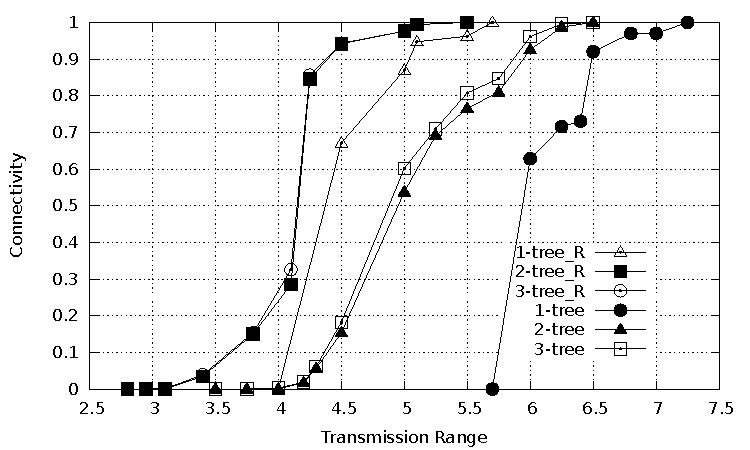
\includegraphics[width=6 in, height=2.6 in]{NetworkI_woR.pdf}
\caption{Connectivity Vs Transmission range for network with relays and network without relays}
\label{Fig:NWOR}
\end{figure}
\subsection{Summary}
\section{ $S-CONN$ Problem}
\subsection{Introduction}
\subsection{Problem Definition}
\begin{defi}[The $Conn(G,\textbf{R},N_{req})$ Problem]
\normalfont
Let $G$ is a UWSN where each node $v\in V$ can be located into a set of regions  $R_v=\{r_{(v,1)},r_{(v,2)},....\}$  with probability $p(r_{(v,i})$ where $i=1,2,...$. Also $R_{tr}(v)$ is the transmission radius for node $v\in V$ and $N_{req}$ is a set of nodes where $N_{req}\subset V$. we would like to find the probability $Conn(G,\textbf{R},N_{req})$ that $N_{req}$ node(s) is connected with the sink node. $\blacksquare$
\end{defi}

\begin{figure}
\centering
\begin{minipage}{.9\linewidth}
\end{minipage}
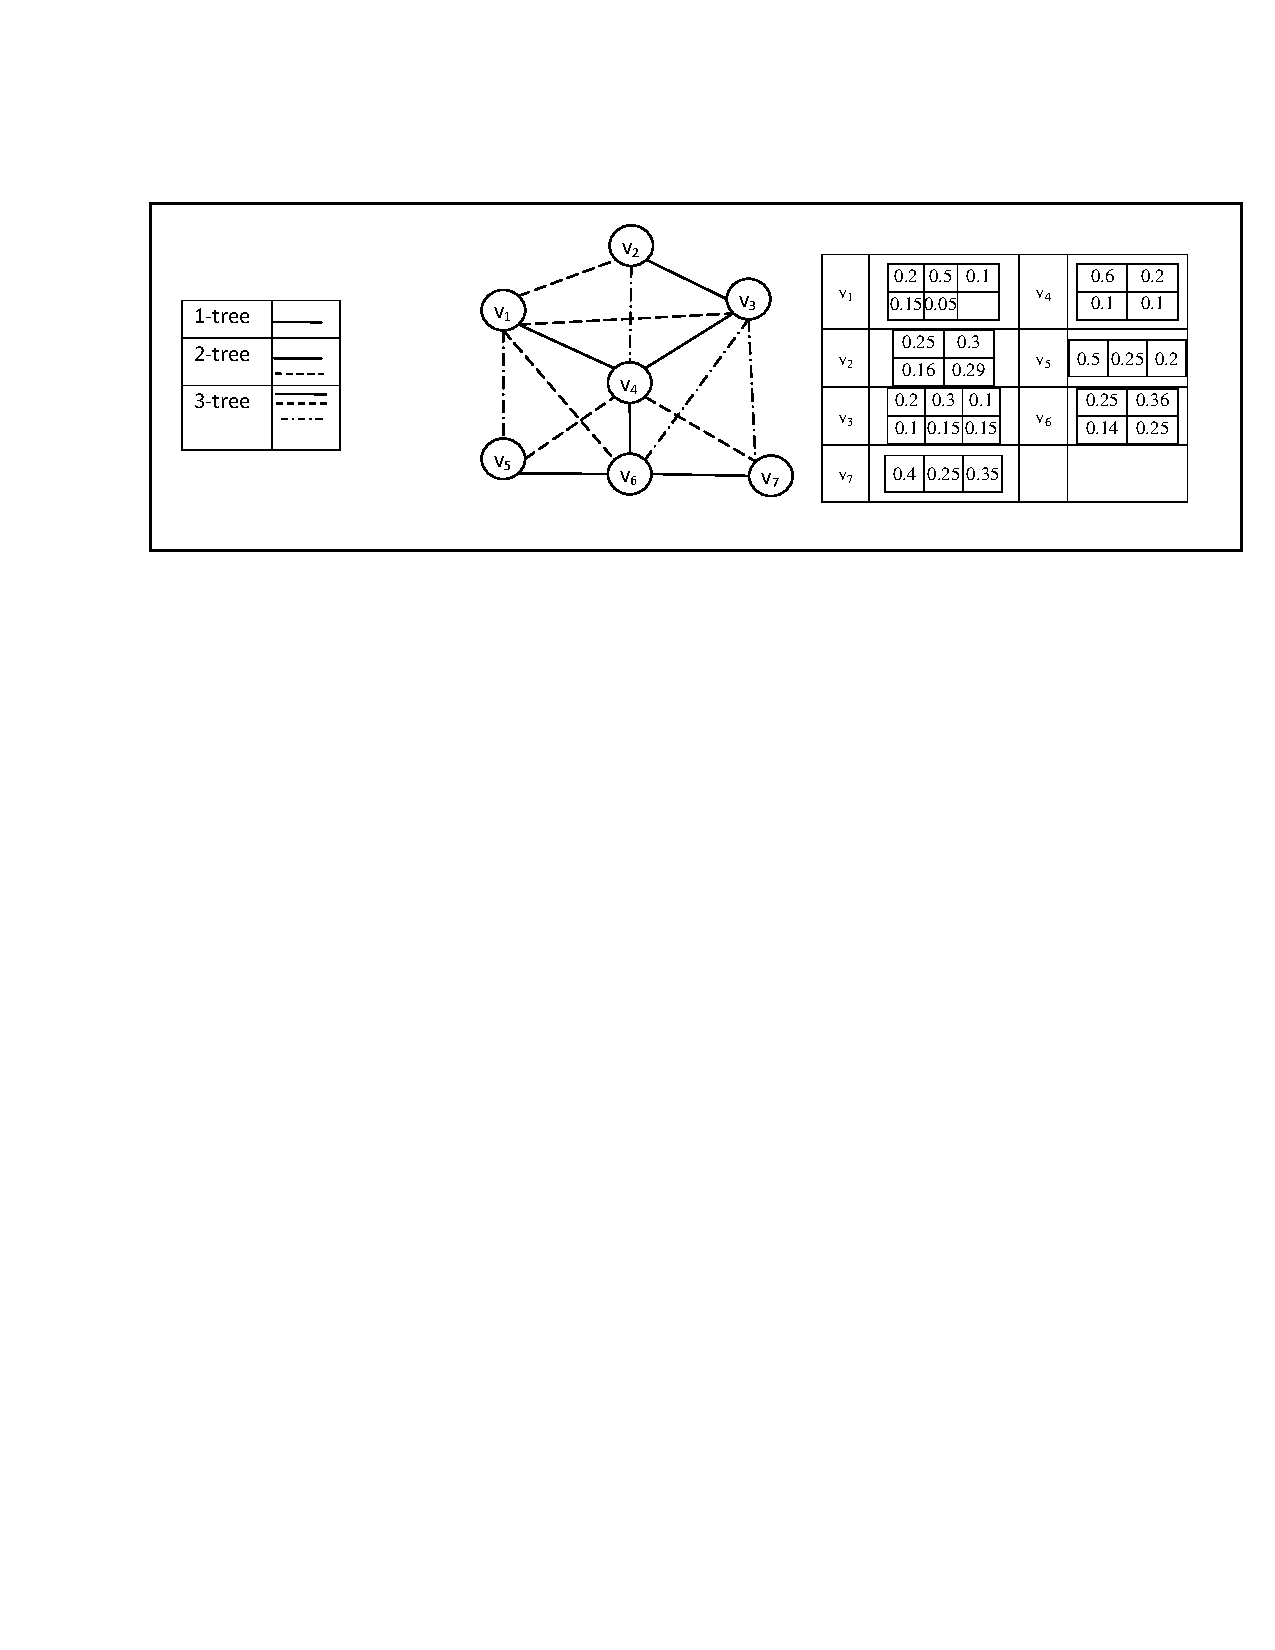
\includegraphics[width=5.5 in, height=1.8 in]{NReq.pdf}
\caption{A partial $3$-tree with $7$ nodes}
\label{Fig:Nreq}
\end{figure}

\begin{exmp}
\normalfont
Fig. \ref{Fig:Nreq} illustrates a network of $7$ nodes. Locality set of nodes $v_1,v_2,v_3,v_4,v_5,v_6$ and $v_7$ has $5,4,6,3,4,3$ and $4$ regions. We are also considering $v_4$ as a sink node. Transmission range \(R_{tr}=8.5\) unit. By using this transmission range, we are interested to find out what is the probability that $N_{req}$ number of nodes including the sink node is connected. For example we are interested to find out what is the probability that $5$ nodes including he sink node is connected. $\blacksquare$
\end{exmp}

\subsection{Algorithms for $S-CONN$}
\subsubsection{Data Structures}
We know from section \ref{subsec:kds} that a typical row in a table is key-value mapping. A key consists of 
i). partitions ii). regional set iii). target node attach and value is the probability. In algorithms for networks with $N_{req}$, we added a new data structure called component size, $Csize$. We are going to explain component size in this section.\\
\textbf{Component Size:} Component size is associated with every partition. Component size of a partition indicates the number of nodes connected with  that partition. Component size of a partition is incremented by one when a node is deleted from that partition. For example if ${\{v_1,v_2,v_4\}}^{\{l_1,l_3,l_5\}}_{(tnodeAttach)} [Csize]$ is a typical key where the partition is $\{v_1,v_2,v_4\}$, regional set and target node attach are shown as a superscript and subscript of the partition and we use square brackets. So if we remove   $v_1$ from the partition the new key will be ${\{v_2,v_4\}}^{\{l_3,l_5\}}_{(tnodeAttach)} [Csize+1]$.    Also when two or more partitions merged into one partition, the component size of the newly created partition will be the mathematical sum of the component size of merged partitions. For example consider two  keys ${\{v_1,v_2,v_4\}}^{\{l_1,l_3,l_5\}}_{(tnodeAttach_1)} [Csize_1]$ and ${\{v_1,v_3,v_5\}}^{\{l_4,l_1,l_2\}}_{(tnodeAttach_2)} [Csize_2]$. After merging these two key the newly formed key will be ${\{v_1,v_2,,v_3,v_4,v_5\}}^{\{l_1,l_3,l_1,l_5,l_2\}}_{(tnodeAttach_1 or tnodeAttach_2)} [Csize_1+Csize_2]$


We use three functions $Main()$, $merge()$ and $pMerge()$  for Network with $N_{req}$ in-order to calculate connectivity. For merging two rows we use $pMerge()$ function described in section \ref{subsub:fMpar}. We modified the $merge()$ function which is used for merging two table described in section \ref{subsub:Mrg} and $Main()$ function which is described in section \ref{subsub:Main}. We added component size, $Csize$ with each partition.In this section we are going to describe the steps we added in the $Main()$ function and $merge()$ function.
\subsubsection{Function Main}
In this section we are going to show when and how we incremented the component size. We added step 10 to the $Main$ function which increment the component size when a node is deleted from a partition.

\begin{itemize}[noitemsep]
\item $Step 10:$ when a node is deleted from a partition the component size of that partition is incremented by one. The component size indicates the number of nodes connected with that partition.
\end{itemize}
\begin{algorithm} [h]
\Indm
\KwIn{ a UWSN $G=(V,E)$ is a partial $k$-tree where each node, $v\in V$  can be located into a set of regions $R_v=\{r_{(v,1)},r_{(v,2)}...\}$ with probability,    
  $\{p(r_{(v,1)}),p(r_{(v,2)})...\}$ and $(x,y)\in E$ if $x\in V$ can be located one of it's locality set and $y\in V$ can be located one of it's locality set, so that they reach each other. $PES$ is a perfect elimination sequence $(v_1,v_2,...,v_{n-k})$ of $G$.}
\KwOut{ Prob, a solution to the input instance.}
\textbf {Notation:} $Temp$ is a map from keys to probabilities.\\
%\noline
\Indp
\nl \textbf{Initialize } every clique by  a table.\\
\nl\For{$i=1,2,...,n-k$}
{
 \nl node $v_i$ is associated with $k$-cliques, $K_{(v_i,1)},K_{(v_i,2)},..,K_{(v_i,k)}$ \\
 //$T_{(v_i,1)},T_{(v_i,2)},..,T_{(v_i,k)}$ are the tables associated with cliques $K_{(v_i,1)},K_{(v_i,2)},..,K_{(v_i,k)}$ respectively \\
\nl $ Temp=T_{(v_i,1)}$  \\
 \nl \For{$j=2,3..,k$}
 {
  \nl $Temp=merge(Temp,T_{(v_i,j)})$\\
 }
 // clique $K_{(v_i,base)}$ is the base clique and table $T_{(v_i,base)}$ is the base table of node $v_i$
  \nl $Temp=merge(Temp,T_{(v_i,base)})$\\
\nl  \If{$v_i$ is in a partition of $Temp$ by itself}{
\nl ignore the row containing that partition.}

 \Else {
\nl increment the component size $Csize$ from the partition containing $v_i$ from $Temp$ and remove node $v_i$ from that partition.\\ 
\nl assign the result to $T_{(v_i,base)}$}
}

\nl \Return{Prob=$\sum$(All probability for single partition in the remaining table)}
\caption{Function Main$(G$, $\textbf{R}$, $p(r_{(v,i)})$, $PES )$}
\end{algorithm}
\subsubsection{Function Merge}
In this section steps 6 and 7 are added with the merge function which is mainly described in section \ref{subsub:Mrg}
\begin{itemize}[noitemsep]
\item $Step 6:$ iterates through each partition, $Par_i$ of newly created array row, $Obj$ where $i=1,2,3,...$. Row $Obj$ is created from row $r$ and row $s$.
\item $Step 7:$ search for a partition(s) $Par_1$ in row $r$ and $Par_2$ in row $s$ where $Par_1\subseteq Par_i$ and  $Par_2\subseteq Par_i$. Finally it calculates the component size for partition $Par_i$  by adding the component size of $Par_1$ and $Par_2$.
\end{itemize}

\begin{algorithm}[H]

\Indm  
\KwIn{ Two tables $T_1$ and $T_2$ that share at least one common vertex}
\KwOut{A  table $T$}

\textbf{Notation} $C$ is a set of vertices and $Obj$ is a row of table $T$ and $Prob\_C$ is a double variable\\
\Indp
\nl \textbf{set} $C=$ the set of common vertices between $T_1$ and $T_2$ , set $Prob\_C=1$\\
 \nl \If{$C\neq \emptyset$}{
 \nl \ForEach{row $r$ in $T_1$}
 {
 \nl \ForEach{row $s$ in $T_2$}
 {
  \nl  $Obj.par=$pMerge($r.par$,$s.par$)\\
  \nl \ForEach{partition $Par_i$ in $Obj.par$ where $i=1,2,3,...$}
    {
   \nl $Obj.Csize[Par_i]=r.Csize[Par1]+s.Csize[Par2]$\\
    //If there is partition $Par1$ in $r$ and $Par2$ in $s$ where $Par1\subseteq Par_i$ and $Par2\subseteq Par_i$
    }
   \nl \ForEach{vertex $v_i$ in $Obj.par$ where $i=1,2,..,k+1$}
    {
   \nl $Obj.loc[v_i]=r.loc[v_i]||s.loc[v_i]$\\
    }
    
   \nl \ForEach{vertex  $v\in C$}
    {
   \nl $Prob\_C=Prob\_C*s.loc[v]$
    }
\nl $ Obj<Obj.par:Obj.loc>=\frac{Prob[r]\times Prob[s]}{Prob\_C}$\\
\nl Insert $Obj$ in $T$ as a row.\\
}
  }
  }
\nl \Return {Table T}

 \caption{Function merge($T_1,T_2$)}
\end{algorithm}

\subsection{Simulation Results}
In this section we used Network I depicted in section \ref{fig:NTRK}. Network I has 10 nodes and each node has a regional set range from 3 to 6. Figure \ref{fig:CVC} depict how connectivity changes with component size.We used $Tx=8$ for transmission range. Also we compare the performance of 1-tree, 2-tree and 3-tree. The graph shows that the connectivity for all trees declining with increasing of component size. Incrementing the component size means we wanted more node should be connected with the sink. As a result the connectivity is declining.  Also we can see that connectivity for 1-tree is declining quickly in comparison with other 2 trees.
\begin{figure}
\begin{minipage}{.9\linewidth}
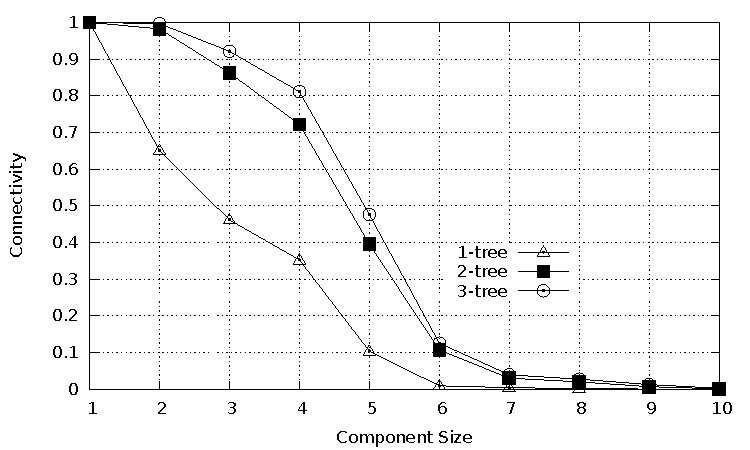
\includegraphics[width=6 in, height=2.8 in]{ConVsCom_woR.pdf}
\caption{Connectivity versus component size for Newtork I }
\label{Fig:CVC}
\end{minipage}
\end{figure}
\subsection{Summary}

\section{ $S-CONN$ with Relays Problem}
\subsection{Introduction}
\subsection{Algorithms for $S-CONN$ with Relays}
\subsubsection{Data Structure}

\subsubsection{Function Main}
\begin{algorithm} [H]
\Indm
\KwIn{ a UWSN $G=(V,E)$ is a partial $k$-tree where each node, $v\in V$  can be located into a set of regions $R_v=\{r_{(v,1)},r_{(v,2)}...\}$ with probability,    
  $\{p(r_{(v,1)}),p(r_{(v,2)})...\}$ and $(x,y)\in E$ if $x\in V$ can be located one of it's locality set and $y\in V$ can be located one of it's locality set, so that they reach each other. A set of target nodes $Tar=\{v_1,v_2,...\}$ where $Tar\subset V$. A set of relay nodes $Rel=\{v_1,v_2,...\}$ where $Rel\subset V$. $PES$ is a perfect elimination sequence $(v_1,v_2,...,v_{n-k})$ of $G$.}
\KwOut{ Prob, a solution to the input instance.}
\textbf {Notation:} $Temp$ is a map from keys to probabilities.\\
%\noline
\Indp
\nl \textbf{Initialize } every clique by  a table.\\
\nl\For{$i=1,2,...,n-k$}
{
 \nl node $v_i$ is associated with $k$-cliques, $K_{(v_i,1)},K_{(v_i,2)},..,K_{(v_i,k)}$ \\
 //$T_{(v_i,1)},T_{(v_i,2)},..,T_{(v_i,k)}$ are the tables associated with cliques $K_{(v_i,1)},K_{(v_i,2)},..,K_{(v_i,k)}$ respectively \\
\nl $ Temp=T_{(v_i,1)}$  \\
 \nl \For{$j=2,3..,k$}
 {
  \nl $Temp=merge(Temp,T_{(v_i,j)})$\\
 }
 // clique $K_{(v_i,base)}$ is the base clique and table $T_{(v_i,base)}$ is the base table of node $v_i$\\
  \nl $Temp=merge(Temp,T_{(v_i,base)})$\\
\nl \If{$v_i$ is in a partition by itself}{
\nl ignore the row containing that partition\\
}
\nl \ElseIf{$v_i$ is a relay node}{
\nl Remove $v_i$ from all the partitions of $Temp$ and assign the result to $T_{(v_i,base)}$ after updating the regional set.\\
}
\Else{
\nl Remove $v_i$ from all the partitions of $Temp$ and increment the component size of corresponding partition by one.\\
\nl  assign the result to $T_{(v_i,base)}$ after updating the regional set.
}
}

\nl \Return{Prob=$\sum$(All probability for single partition in the remaining table)}
\caption{Function Main$(G$, $\textbf{R}$, $Tar$, $Rel$, $p(r_{(v,i)})$, $PES )$}
\end{algorithm}
\subsubsection{Function Merge}
\begin{algorithm}[H]
\Indm  
\KwIn{ Two tables $T_1$ and $T_2$ that share at least one common vertex}
\KwOut{A  table $T$}

\textbf{Notation} $C$ is a set of vertices and $Obj$ is a row of table $T$ and $Prob\_C$ is a double variable\\
\Indp
\nl \textbf{set} $C=$ the set of common vertices between $T_1$ and $T_2$ , set $Prob\_C=1$\\
 \nl \If{$C\neq \emptyset$}{
 \nl \ForEach{row $r$ in $T_1$}
 {
 \nl \ForEach{row $s$ in $T_2$}
 {
  \nl  $Obj.par=$pMerge($r.par$,$s.par$)\\
  \nl \ForEach{partition $Par_i$ in $Obj.par$ where $i=1,2,3,...$}
    {
   \nl $Obj.Csize[Par_i]=r.Csize[Par1]+s.Csize[Par2]$\\
    //If there is partition $Par1$ in $r$ and $Par2$ in $s$ where $Par1\subseteq Par_i$ and $Par2\subseteq Par_i$
    }
   \nl \ForEach{vertex $v_i$ in $Obj.par$ where $i=1,2,..,k+1$}
    {
   \nl $Obj.locmap[v_i]=r.locmap[v_i]||s.locmap[v_i]$\\
    }
    \nl \ForEach{node $v$ in every partition $P$ in $Obj.par$}
    {
    \nl \ForEach{node $u$ in every partition $Q$ in $s.par$}
    {
    \nl \If{$v==u$}
    {
   \nl $Obj.tAttach[P]=max(Obj.tAttach[P],s.tAttach[Q])$
    }
    }
    
     \nl \ForEach{node $w$ in every partition $T$ in $r.par$}
    {
    \nl \If{$v==w$}
    {
    \nl $Obj.tAttach[P]=max(Obj.tAttach[P],r.tAttach[T])$
    }
    }
    }
   \nl \ForEach{vertex  $v\in C$}
    {
   \nl $Prob\_C=Prob\_C*s.loc[v]$
    }
\nl $ Obj<Obj.par:Obj.loc>=\frac{Prob[r]\times Prob[s]}{Prob\_C}$\\
\nl Insert $Obj$ in $T$ as a row.\\
}
  }
  }
\nl \Return {Table T}

 \caption{Function merge($T_1,T_2$)}
\end{algorithm}
\subsection{Simulation Results}

\subsection{Summary}



% ------------------------------------------------------------
%\section{ References}
\bibliographystyle{plain} 
\bibliography{ThesisWriteup}
% ------------------------------------------------------------
%\hLine{2 in}
\end{document}
